本节基于四个公开电池数据集对所提 MS-AgentNet 模型进行系统性评估。研究设置多组验证实验，主要包含健康指标有效性验证、模型性能对比分析、模块消融与复杂度评估以及跨域适应性测试。其中，健康指标有效性实验用于验证所选特征对电池退化模式的表征能力，可有效评价模型输入的合理性；模型对比实验用于检验所提方法在跨电池场景下的估计精度与稳定性；通过消融实验与复杂度分析可量化核心模块的贡献程度，并评估模型的计算效率；最终通过跨数据集迁移实验进一步考察模型对数据域差异的适应能力。综合上述多维度实验结果，可全面验证所提 MS-AgentNet 模型在电池 SOH 估计任务中的有效性与适用性。

\subsection{评价指标}

为评价模型的 SOH 估计性能，选取平均绝对误差（MAE）、平均绝对百分比误差（MAPE）、均方根误差（RMSE）和决定系数（R²）四项常用指标\cite{ref76}。

MAE 表示全部评价样本中预测 SOH 与真实 SOH 之间绝对误差的平均值，用于反映模型的整体误差水平。该指标不会进一步放大单个较大偏差，能够较为直观地衡量总体估计精度。

MAPE 通过真实 SOH 对绝对误差进行归一化，便于比较不同数据集上的估计性能。当真实 SOH 接近零时，MAPE 可能被显著放大，需结合 MAE 和 RMSE 进行综合评价。

RMSE 表示预测 SOH 与真实 SOH 之间均方误差的平方根。与 MAE 相比，RMSE 对较大的预测偏差赋予更高权重，可以进一步反映模型对较大误差的控制能力。

R² 衡量模型对真实 SOH 变化的拟合程度，其值越接近 1，表明模型对整体退化趋势的拟合效果越好。

上述四项指标的数学定义如下：

\begin{equation}
\label{eq:metric_mae}
\mathrm{MAE}=\frac{1}{n}\sum_{i=1}^{n}\left|y_i-\hat{y}_i\right|
\end{equation}

\begin{equation}
\label{eq:metric_mape}
\mathrm{MAPE}=\frac{1}{n}\sum_{i=1}^{n}\left|\frac{y_i-\hat{y}_i}{y_i}\right|
\end{equation}

\begin{equation}
\label{eq:metric_rmse}
\mathrm{RMSE}=\sqrt{\frac{1}{n}\sum_{i=1}^{n}\left(y_i-\hat{y}_i\right)^2}
\end{equation}

\begin{equation}
\label{eq:metric_r2}
R^2=1-\frac{\sum_{i=1}^{n}\left(y_i-\hat{y}_i\right)^2}{\sum_{i=1}^{n}\left(y_i-\bar{y}\right)^2}
\end{equation}

其中，$y_i$ 和 $\hat{y}_i$ 分别表示第 $i$ 个样本的真实 SOH 和预测 SOH，$\bar{y}$ 表示评价样本中真实 SOH 的平均值，$n$ 表示评价样本总数。

\subsection{健康指标筛选结果与有效性分析}

为验证组级健康指标筛选方法在识别跨电池稳定输入方面的有效性，本节以 Oxford 数据集为例比较不同健康指标输入下的 SOH 估计性能。根据 Cell1 上候选指标的 PCC 和 SCC，从 IC、DTV 和 DTC 三类特征中各选取一项综合相关性最高的指标，分别为 HI4、HI9 和 HI11，三者的综合相关性得分均高于 0.94。将上述指标与组级筛选得到的 CCCT 指标 HI1 分别输入 MS-AgentNet，并将 HI1、HI4、HI9 和 HI11 共同输入的方案记为 Fusion。不同输入下 Cell2--Cell8 的 SOH 估计结果见\cref{tab:4-hi-input}。

结果表明，HI1 在 Cell2--Cell8 上始终保持较高的估计精度，其平均 MAE、RMSE 和 MAPE 均为五种输入方案中的最低值，平均 MAPE 为 0.00615，即 0.615\%。当四项健康指标共同作为输入时，Fusion 的三项平均误差均排名第四，说明多类健康指标的直接组合没有形成进一步的性能增益。

此外，同一健康指标的表征能力在不同电池间存在差异。例如，HI9 在 Cell7 上的估计误差低于 HI11，而在 Cell8 上则观察到相反结果。相比之下，组级筛选得到的 HI1 在七节电池上均取得最低的 MAE、RMSE 和 MAPE。上述结果表明，单节电池上的高相关性不能保证健康指标在组内其他电池上保持相同的表征能力，而组级筛选得到的 HI1 在该组 Oxford 电池上提供了更稳定的 SOH 估计输入。
\begin{table}[H]
\TableStyle
\fontsize{7.5pt}{9.5pt}\selectfont
\setlength{\tabcolsep}{1.5pt}
\renewcommand{\arraystretch}{1.18}
\caption{SOH estimation errors of different health-indicator inputs on the Oxford dataset.}
\label{tab:4-hi-input}
\begin{tabular*}{\linewidth}{@{\extracolsep{\fill}}l*{15}{c}@{}}
\toprule
& \multicolumn{5}{c}{MAE (\%)}
& \multicolumn{5}{c}{RMSE (\%)}
& \multicolumn{5}{c}{MAPE (\%)} \\
\cmidrule(lr){2-6}\cmidrule(lr){7-11}\cmidrule(lr){12-16}
Cell
& IC & CCCT & DTV & DTC & Fusion
& IC & CCCT & DTV & DTC & Fusion
& IC & CCCT & DTV & DTC & Fusion \\
\midrule
Cell2
& 0.70 & \textbf{\underline{0.43}} & 1.71 & 4.84 & 1.61
& 0.98 & \textbf{\underline{0.69}} & 2.08 & 5.62 & 1.97
& 0.87 & \textbf{\underline{0.52}} & 2.01 & 5.85 & 1.91 \\
Cell3
& 0.45 & \textbf{\underline{0.28}} & 9.85 & 11.40 & 2.28
& 0.52 & \textbf{\underline{0.35}} & 10.42 & 12.86 & 2.64
& 0.53 & \textbf{\underline{0.33}} & 11.32 & 13.89 & 2.66 \\
Cell4
& \textbf{\underline{0.58}} & 0.81 & 1.26 & 2.77 & 1.28
& \textbf{\underline{0.74}} & 0.87 & 1.46 & 3.73 & 1.62
& \textbf{\underline{0.69}} & 0.96 & 1.44 & 3.12 & 1.44 \\
Cell5
& 0.73 & \textbf{\underline{0.30}} & 2.61 & 9.39 & 1.82
& 0.79 & \textbf{\underline{0.35}} & 3.63 & 10.07 & 2.16
& 0.82 & \textbf{\underline{0.34}} & 2.86 & 10.58 & 2.04 \\
Cell6
& 0.87 & \textbf{\underline{0.59}} & 1.27 & 7.23 & 2.22
& 1.16 & \textbf{\underline{0.84}} & 1.61 & 8.64 & 2.55
& 1.00 & \textbf{\underline{0.71}} & 1.43 & 7.99 & 2.52 \\
Cell7
& 1.67 & \textbf{\underline{0.80}} & 1.25 & 6.10 & 1.91
& 1.71 & \textbf{\underline{0.83}} & 1.54 & 7.42 & 2.07
& 1.91 & \textbf{\underline{0.92}} & 1.41 & 6.83 & 2.18 \\
Cell8
& 1.22 & \textbf{\underline{0.39}} & 2.05 & 7.92 & 3.38
& 1.32 & \textbf{\underline{0.47}} & 2.35 & 9.08 & 3.86
& 1.41 & \textbf{\underline{0.44}} & 2.41 & 8.97 & 3.87 \\
\addlinespace[2pt]
Average
& 0.89 & \textbf{\underline{0.52}} & 2.86 & 7.09 & 2.07
& 1.03 & \textbf{\underline{0.63}} & 3.30 & 8.20 & 2.41
& 1.03 & \textbf{\underline{0.61}} & 3.27 & 8.17 & 2.37 \\
\bottomrule
\end{tabular*}
\end{table}


\subsection{模型训练鲁棒性与超参数分析}

为进一步考察 MS-AgentNet 的训练稳定性及轻量化模型的参数设置，本文对智能体矩阵的初始化策略、模型收敛表现和超参数配置进行分析。

\subsubsection{智能体矩阵初始化与收敛性分析}

RAA 将智能体表示为与输入无关的静态可学习矩阵 $\mathbf A\in\mathbb R^{n_a\times d}$，用于全局特征聚合，智能体数量固定为 $n_a=2$。矩阵参数采用均值为 0、标准差为 0.02 的正态分布初始化：

\begin{equation}
\label{eq:agent_initialization}
A_{ij}\sim\mathcal N\!\left(0,0.02^2\right)
\end{equation}

式中，$A_{ij}$ 表示第 $i$ 个智能体在第 $j$ 维特征上的参数。该初始化能够为不同智能体提供幅值较小且非一致的初始参数，避免其处于完全相同的初始状态。

三种初始化方案的对比结果如\cref{tab:4-3-initialization}所示。各方案对应的 $R^2$ 为 0.98527～0.98645，RMSE 为 0.00774～0.00805，MAE 为 0.00485～0.00499，表明其预测性能较为接近。截断正态通过限定采样范围控制参数幅值，Xavier 均匀初始化则根据网络层的输入和输出维度调整参数方差。相比之下，普通正态初始化能够直接为静态智能体矩阵提供以零为中心的小幅随机参数，且不依赖额外的范围限制或维度缩放。因此，本文采用普通正态初始化作为默认设置。

模型收敛特性通过收敛速度和训练后期损失波动共同评价。将训练损失首次降至首轮损失 10\% 以下的训练轮次定义为收敛阈值轮次，并采用最后 20 轮损失的均值和标准差描述训练后期的收敛状态。如\cref{tab:4-3}所示，各次训练均达到预设收敛阈值。Oxford 和 MIT 数据集上的收敛阈值轮次中位数分别为 26 和 7，训练后期损失标准差中位数分别为 $2.38\times10^{-4}$ 和 $4.84\times10^{-6}$。上述结果表明，MS-AgentNet 在当前实验设置下能够稳定收敛，且训练后期的损失波动较小。

\begin{table}
\TableStyle
\caption{Initialization strategy comparison on the Oxford dataset.}
\label{tab:4-3-initialization}
\begin{tabularx}{\linewidth}{@{\extracolsep{\fill}}L{1.15}C{1.05}C{1.05}C{1.05}C{0.90}C{0.90}C{0.90}@{}}
\toprule
Initialization
& \makecell{Threshold epoch\\median (range)}
& \makecell{Late mean loss\\median}
& \makecell{Late loss std.\\median}
& \makecell{$R^2$\\mean $\pm$ std.}
& \makecell{RMSE\\mean $\pm$ std.}
& \makecell{MAE\\mean $\pm$ std.} \\
\midrule
\makecell[tl]{Normal\\$\mathcal N(0,0.02^2)$}
& 18 (14--22)
& $9.5535\times10^{-4}$
& $2.6246\times10^{-4}$
& \makecell[c]{$0.98606$\\$\pm0.00411$}
& \makecell[c]{$0.00784$\\$\pm0.00116$}
& \makecell[c]{$0.00490$\\$\pm0.00054$} \\
\makecell[tl]{Truncated normal\\($\pm2\sigma$)}
& 18 (13--22)
& $9.4815\times10^{-4}$
& $2.6516\times10^{-4}$
& \makecell[c]{$0.98645$\\$\pm0.00371$}
& \makecell[c]{$0.00774$\\$\pm0.00103$}
& \makecell[c]{$0.00485$\\$\pm0.00048$} \\
Xavier uniform
& 18 (14--22)
& $9.5526\times10^{-4}$
& $2.6340\times10^{-4}$
& \makecell[c]{$0.98527$\\$\pm0.00462$}
& \makecell[c]{$0.00805$\\$\pm0.00126$}
& \makecell[c]{$0.00499$\\$\pm0.00058$} \\
\bottomrule
\end{tabularx}
\TableNote{Note: The three strategies are evaluated under five matched random seeds. Standard deviations are population standard deviations.}
\end{table}

\begin{table}[!htbp]
\caption{Convergence characteristics of MS-AgentNet.}
\label{tab:4-3}
\raggedright
\zihao{-5}
\setlength{\tabcolsep}{2.4pt}
\renewcommand{\arraystretch}{1.04}
\begin{ThreePartTable}
\begin{adjustbox}{max width=\linewidth}
\begin{tabularx}{\linewidth}{>{\raggedright\arraybackslash}p{0.14\linewidth}>{\centering\arraybackslash}p{0.17\linewidth}>{\centering\arraybackslash}p{0.17\linewidth}>{\centering\arraybackslash}p{0.20\linewidth}>{\centering\arraybackslash}p{0.20\linewidth}}
\toprule
数据集 & 10\%阈值轮次中位数 & 阈值轮次范围 & 后期平均损失中位数 & 后期损失标准差中位数 \\
\midrule
Oxford & 26 & 18–35 & $8.14\times10^{-4}$ & $2.38\times10^{-4}$ \\
MIT & 7 & 6–8 & $5.84\times10^{-5}$ & $4.84\times10^{-6}$ \\
\bottomrule
\end{tabularx}
\end{adjustbox}
\begin{tablenotes}[flushleft]
\footnotesize
\item[] \parbox[t]{0.98\linewidth}{Note: Statistics are calculated from runs using five different random seeds. The threshold-epoch range is reported as the minimum--maximum.}
\end{tablenotes}
\end{ThreePartTable}
\end{table}

\FloatBarrier

\subsubsection{超参数配置}

MS-AgentNet 的主要超参数包括学习率、网络深度 $L$ 和嵌入维度 $d$，各参数的配置范围见\cref{tab:4-1}。在上述范围内，各数据集利用特征开发集合中的两节电池完成模型训练和配置，其中一节用于模型参数学习，另一节用于超参数配置。Oxford、CALCE CS2、CALCE CX2 和 MIT/Severson 数据集对应的训练电池与配置电池分别为 Cell1 与 Cell2、CS2\_36 与 CS2\_37、CX2\_36 与 CX2\_37 以及 b3c8 与 b3c13。

五种模型的层配置见\cref{tab:4-4}。

\begin{table}[!htbp]
\caption{Layer configurations of different deep learning models.}
\label{tab:4-4}
\raggedright
\zihao{-5}
\setlength{\tabcolsep}{2.7pt}
\renewcommand{\arraystretch}{1.10}
\newcommand{\cfgsep}{\par\vspace{0.58\baselineskip}}
\begin{ThreePartTable}
\begin{tabularx}{\linewidth}{@{}
  >{\hsize=.96\hsize\raggedright\arraybackslash}X
  >{\hsize=1.10\hsize\raggedright\arraybackslash}X
  >{\hsize=1.03\hsize\raggedright\arraybackslash}X
  >{\hsize=1.18\hsize\raggedright\arraybackslash}X
  >{\hsize=.73\hsize\raggedright\arraybackslash}X@{}}
\toprule
MS-AgentNet & CNN-\newline Transformer & Transformer & CNN-LSTM & LSTM \\
\midrule
\begin{minipage}[t]{\hsize}\vspace{0pt}\raggedright\setlength{\parskip}{0pt}
Input\cfgsep
Embedding layer\newline(16)\cfgsep
SLFA module\cfgsep
DSConv-L module\cfgsep
Add \& Norm\cfgsep
FFN\cfgsep
Add \& Norm\cfgsep
Linear layer
\end{minipage}
&
\begin{minipage}[t]{\hsize}\vspace{0pt}\raggedright\setlength{\parskip}{0pt}
Input\cfgsep
Embedding layer\newline(16)\cfgsep
Positional encoder\cfgsep
Softmax attention\cfgsep
$2\times$ Conv1D + ReLU\cfgsep
MLP\cfgsep
Transformer decoder\cfgsep
Linear layer
\end{minipage}
&
\begin{minipage}[t]{\hsize}\vspace{0pt}\raggedright\setlength{\parskip}{0pt}
Input\cfgsep
Embedding layer\newline(16)\cfgsep
Positional encoder\cfgsep
Softmax attention\cfgsep
Add \& Norm\cfgsep
MLP\cfgsep
Add \& Norm\cfgsep
Transformer decoder\cfgsep
Linear layer
\end{minipage}
&
\begin{minipage}[t]{\hsize}\vspace{0pt}\raggedright\setlength{\parskip}{0pt}
Input\cfgsep
Conv1D + ReLU\cfgsep
MaxPooling1D\cfgsep
$3\times$ Conv1D + ReLU\cfgsep
$3\times$ LSTM layer (16)\cfgsep
Linear layer
\end{minipage}
&
\begin{minipage}[t]{\hsize}\vspace{0pt}\raggedright\setlength{\parskip}{0pt}
Input\cfgsep
Linear layer (16)\cfgsep
$5\times$ LSTM layer (16)\cfgsep
Linear layer
\end{minipage}
\\
\bottomrule
\end{tabularx}
\end{ThreePartTable}
\end{table}


确定后的模型配置保持不变。在后续 SOH 估计性能比较中，MS-AgentNet 采用学习率 0.001、网络深度 $L=1$ 和嵌入维度 $d=16$。

\begin{table}
\TableStyle
\caption{Hyperparameter search space of MS-AgentNet.}
\label{tab:4-1}
\begin{tabularx}{\linewidth}{@{\extracolsep{\fill}}L{0.90}L{1.10}@{}}
\toprule
超参数 & 搜索空间 \\
\midrule
学习率 & 0.001, 0.01 \\
网络深度 $L$ & 1, 2, 4, 8 \\
嵌入维度 $d$ & 16, 32, 64, 128 \\
全连接层维度 & 16, 32, 64, 128 \\
\bottomrule
\end{tabularx}
\end{table}


\subsection{SOH估计精度与跨电池泛化性能比较}

根据第~2.3~节的筛选结果，Oxford 数据集采用 HI1，CALCE CS2 数据集采用 HI1 和 HI2，CALCE CX2 数据集采用 HI13，MIT/Severson 数据集采用 HI14 和 HI15。在上述健康指标输入下，进一步比较 MS-AgentNet 与四种基线模型的 SOH 估计性能。


\subsubsection{Oxford数据集上的估计精度分析}

\Cref{fig:4-2}和\cref{tab:4-5}展示了 MS-AgentNet、CNN-Transformer、CNN-LSTM、Transformer 和 LSTM 在 Oxford Cell2--Cell8 上的 SOH 估计结果和误差。

\begin{figure}[htbp]
\centering
\makebox[\textwidth][c]{%
\begin{minipage}{18.5cm}\centering
\begin{minipage}[t]{0.326\textwidth}\centering
{\fontsize{10}{12}\selectfont\bfseries Cell2}\\[-0.1em]
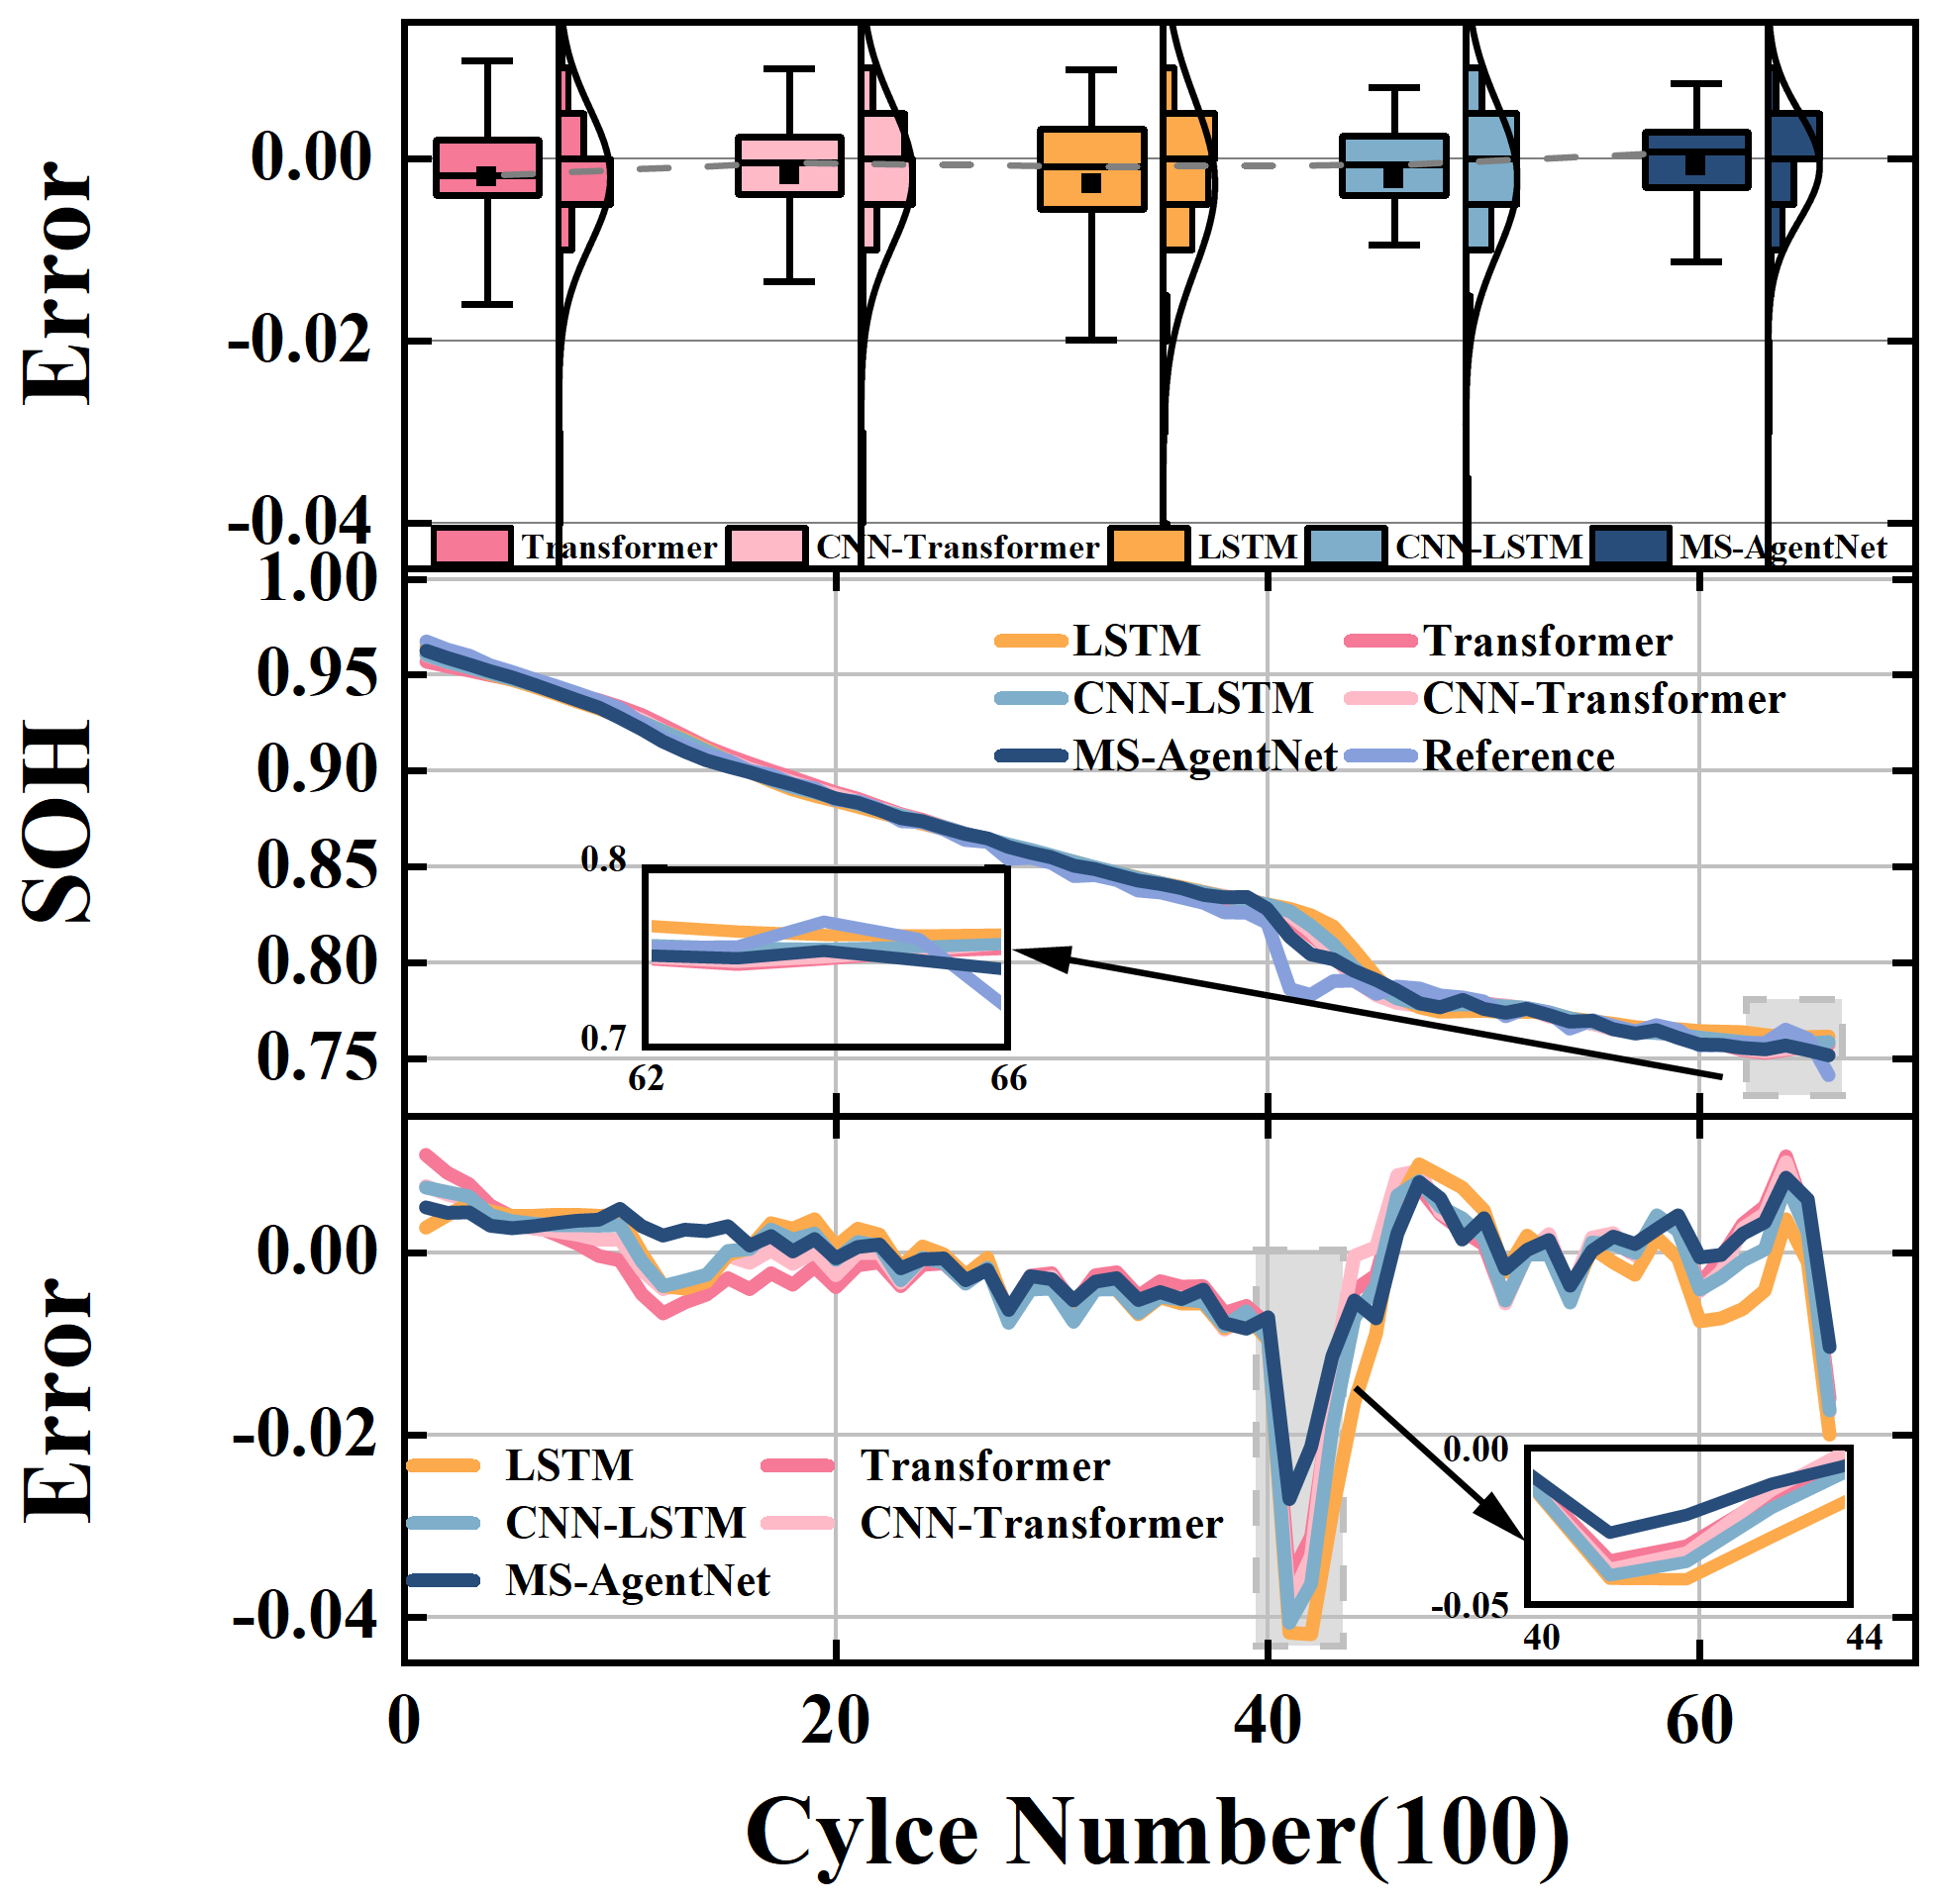
\includegraphics[width=\linewidth]{figures/Oxford/cell2.png}
\end{minipage}%
\hspace{0.01\textwidth}%
\begin{minipage}[t]{0.326\textwidth}\centering
{\fontsize{10}{12}\selectfont\bfseries Cell3}\\[-0.1em]
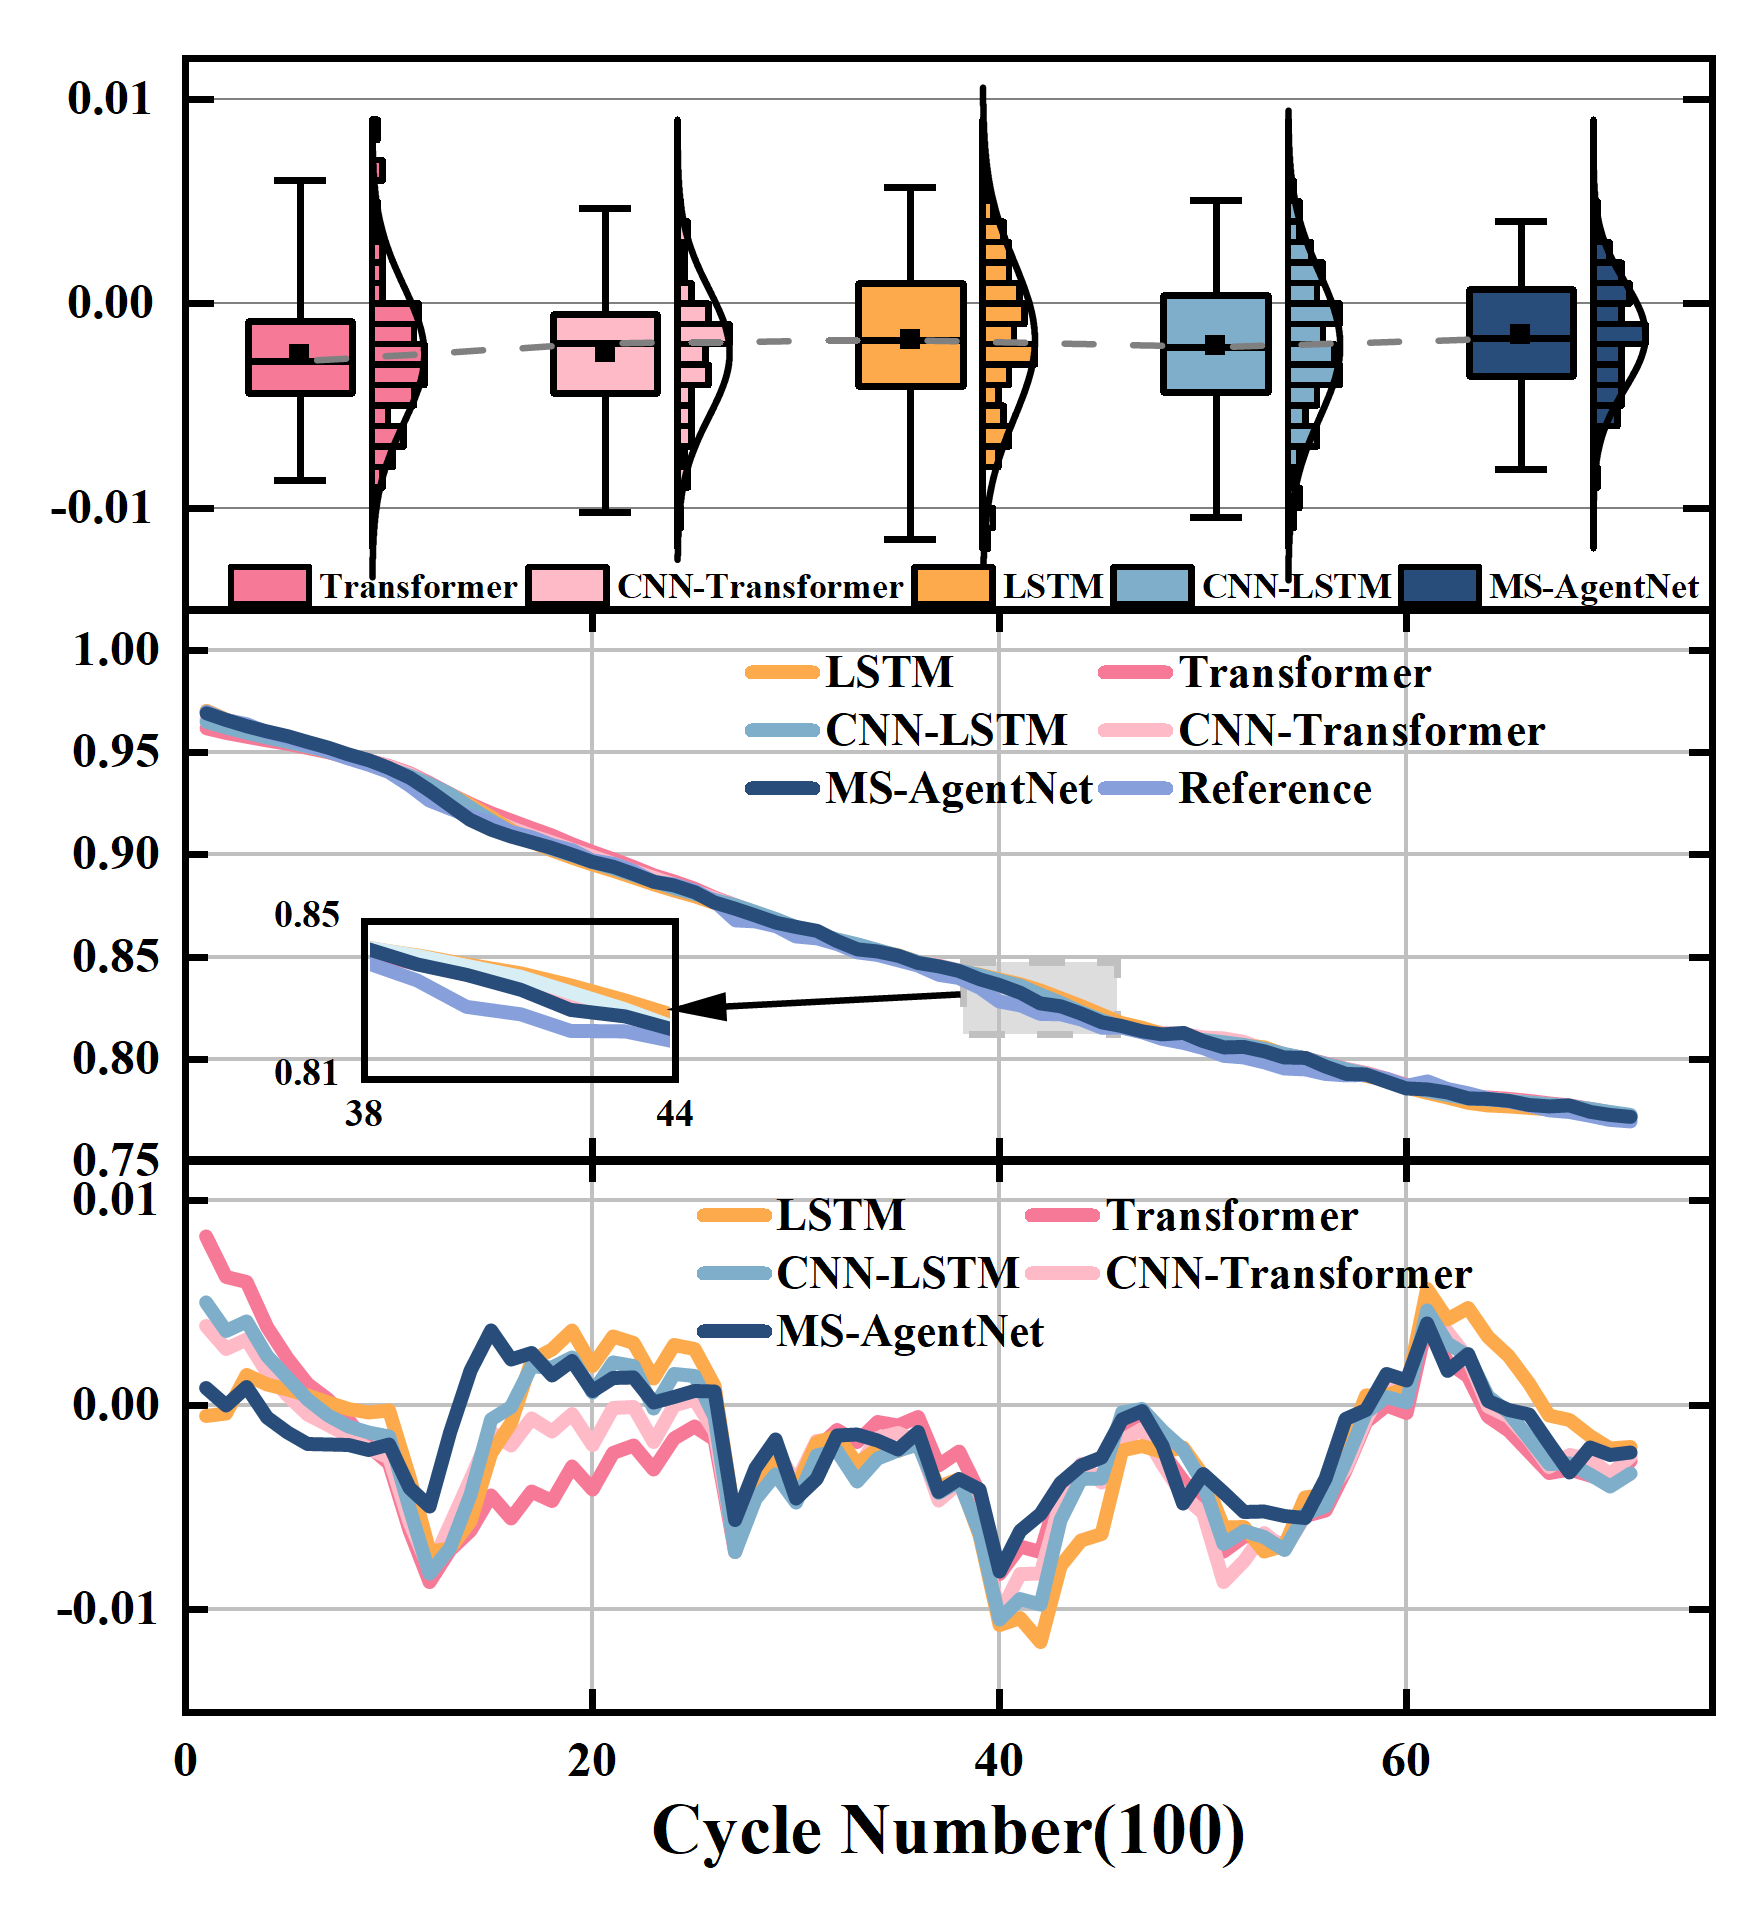
\includegraphics[width=\linewidth]{figures/Oxford/cell3.png}
\end{minipage}%
\\[0.7em]
\begin{minipage}[t]{0.326\textwidth}\centering
{\fontsize{10}{12}\selectfont\bfseries Cell4}\\[-0.1em]
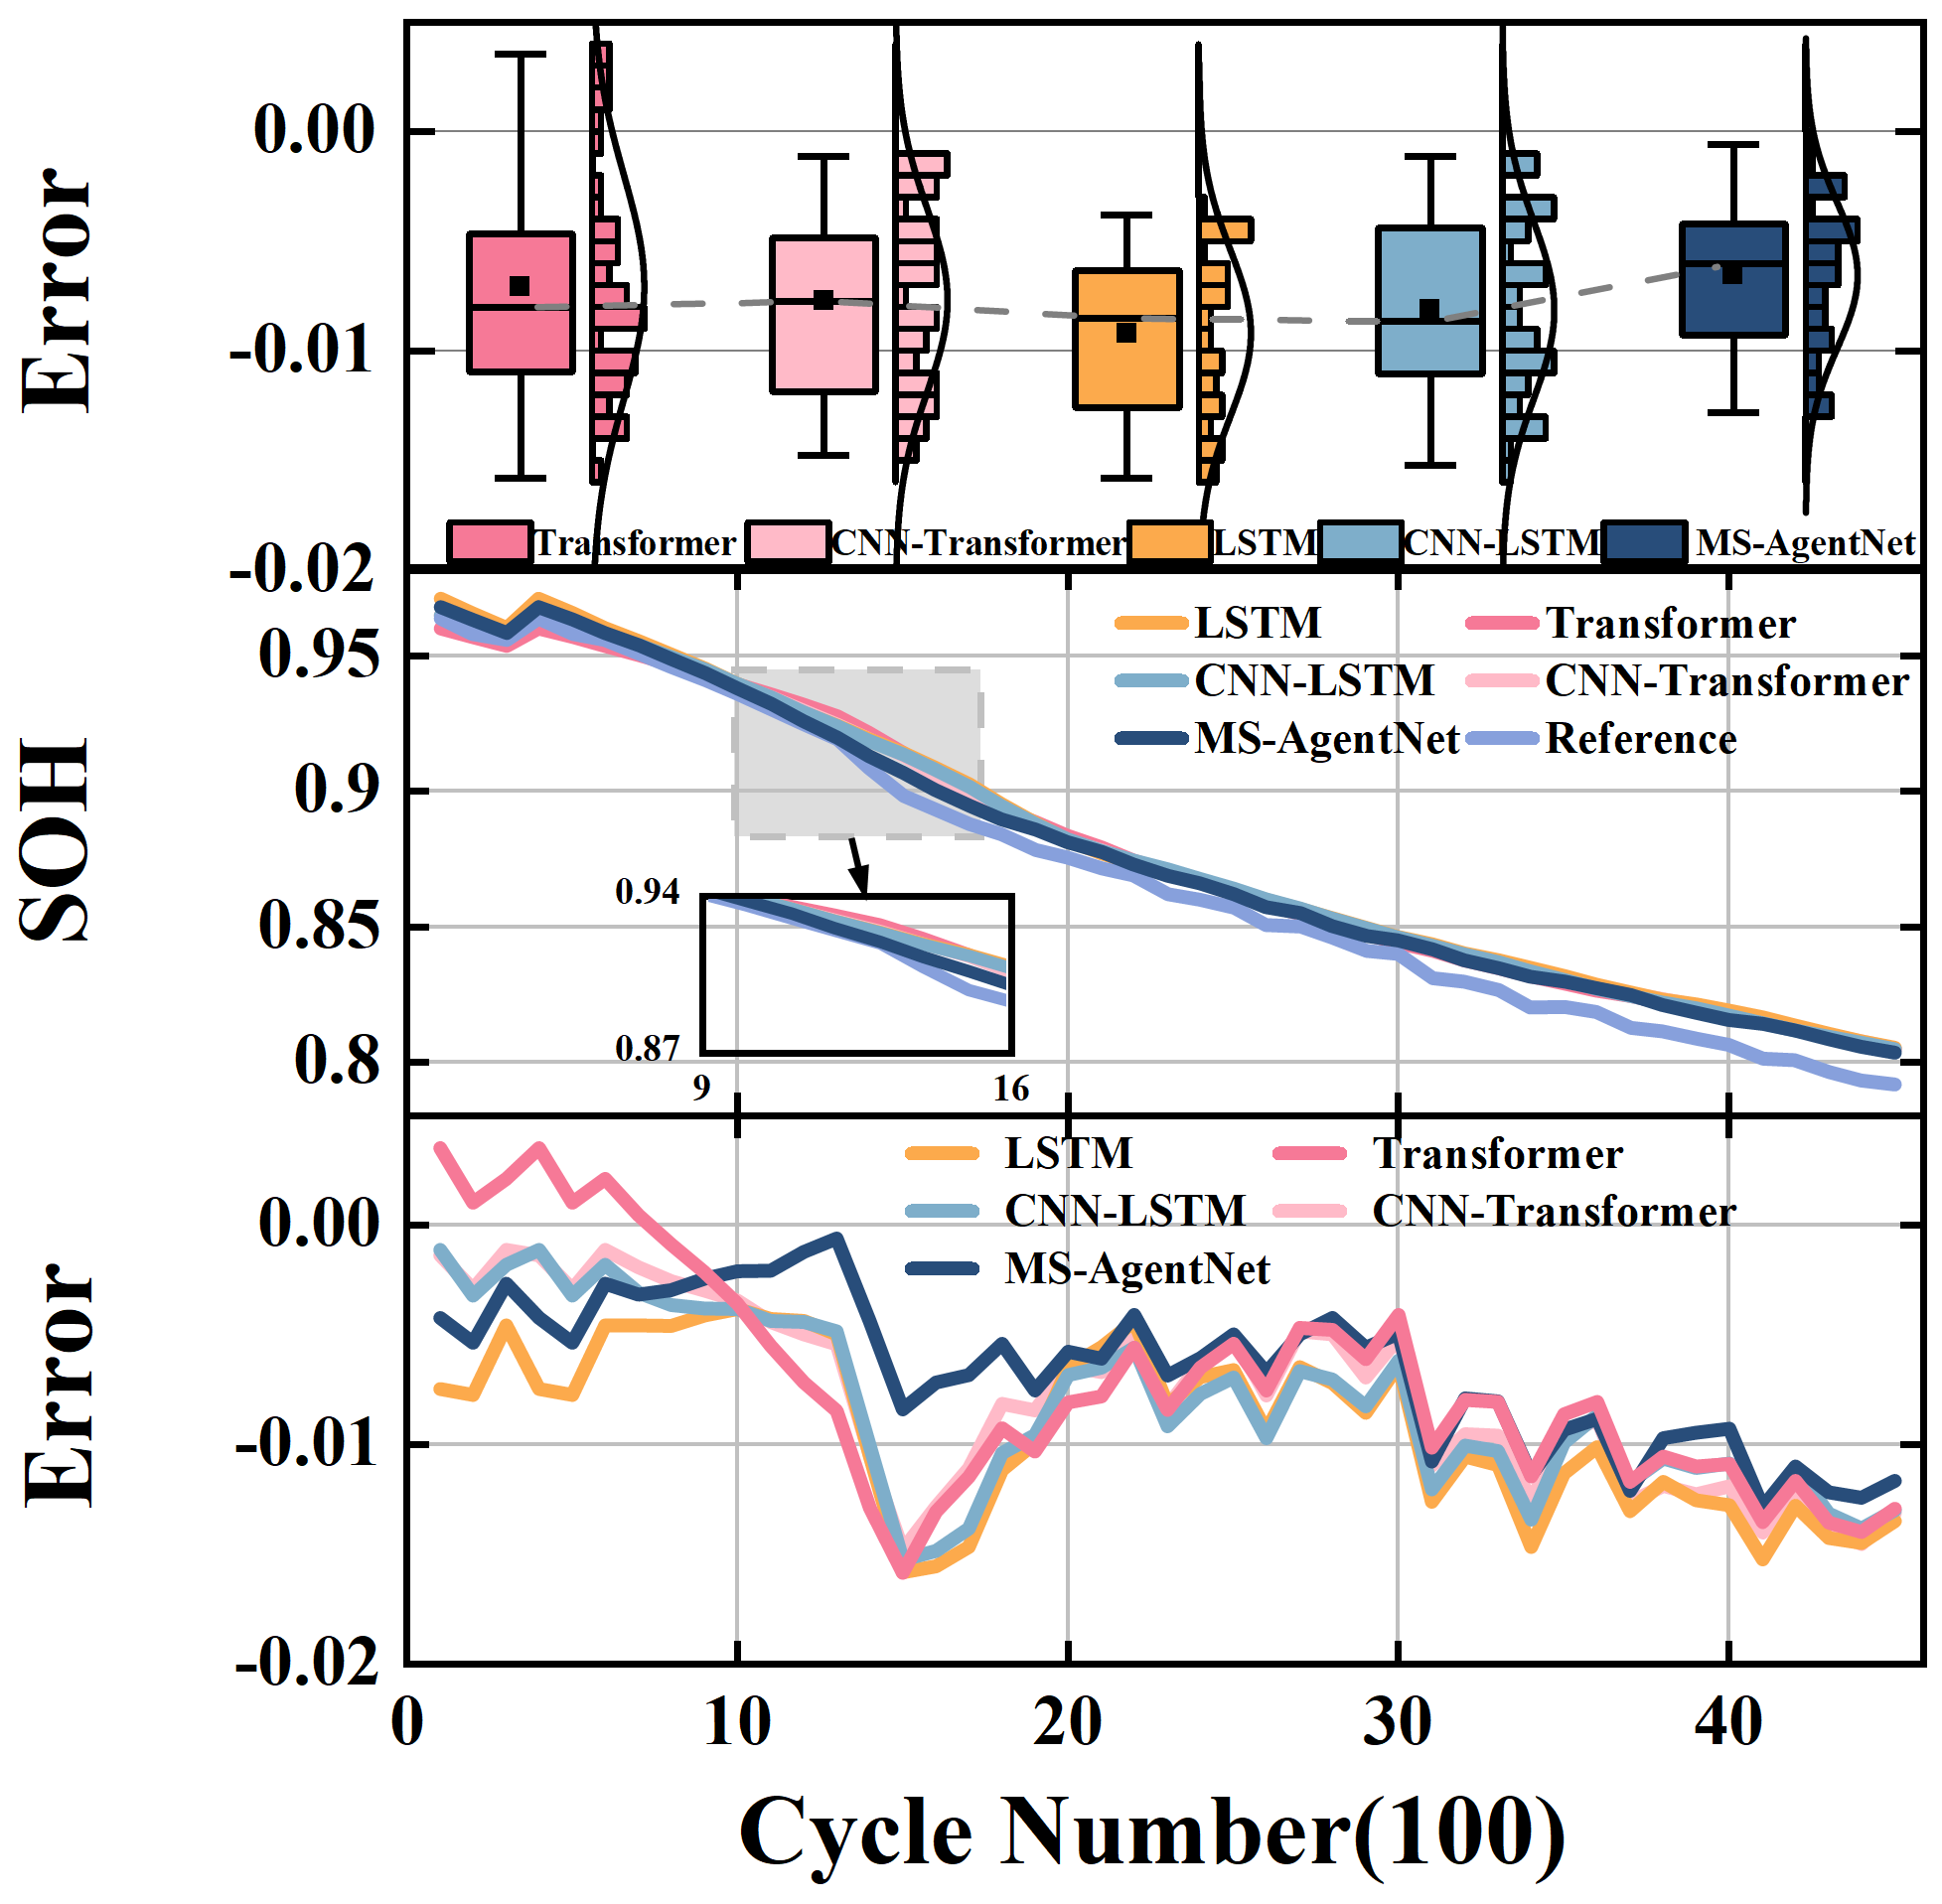
\includegraphics[width=\linewidth]{figures/Oxford/cell4.png}
\end{minipage}%
\hspace{0.01\textwidth}%
\begin{minipage}[t]{0.326\textwidth}\centering
{\fontsize{10}{12}\selectfont\bfseries Cell5}\\[-0.1em]
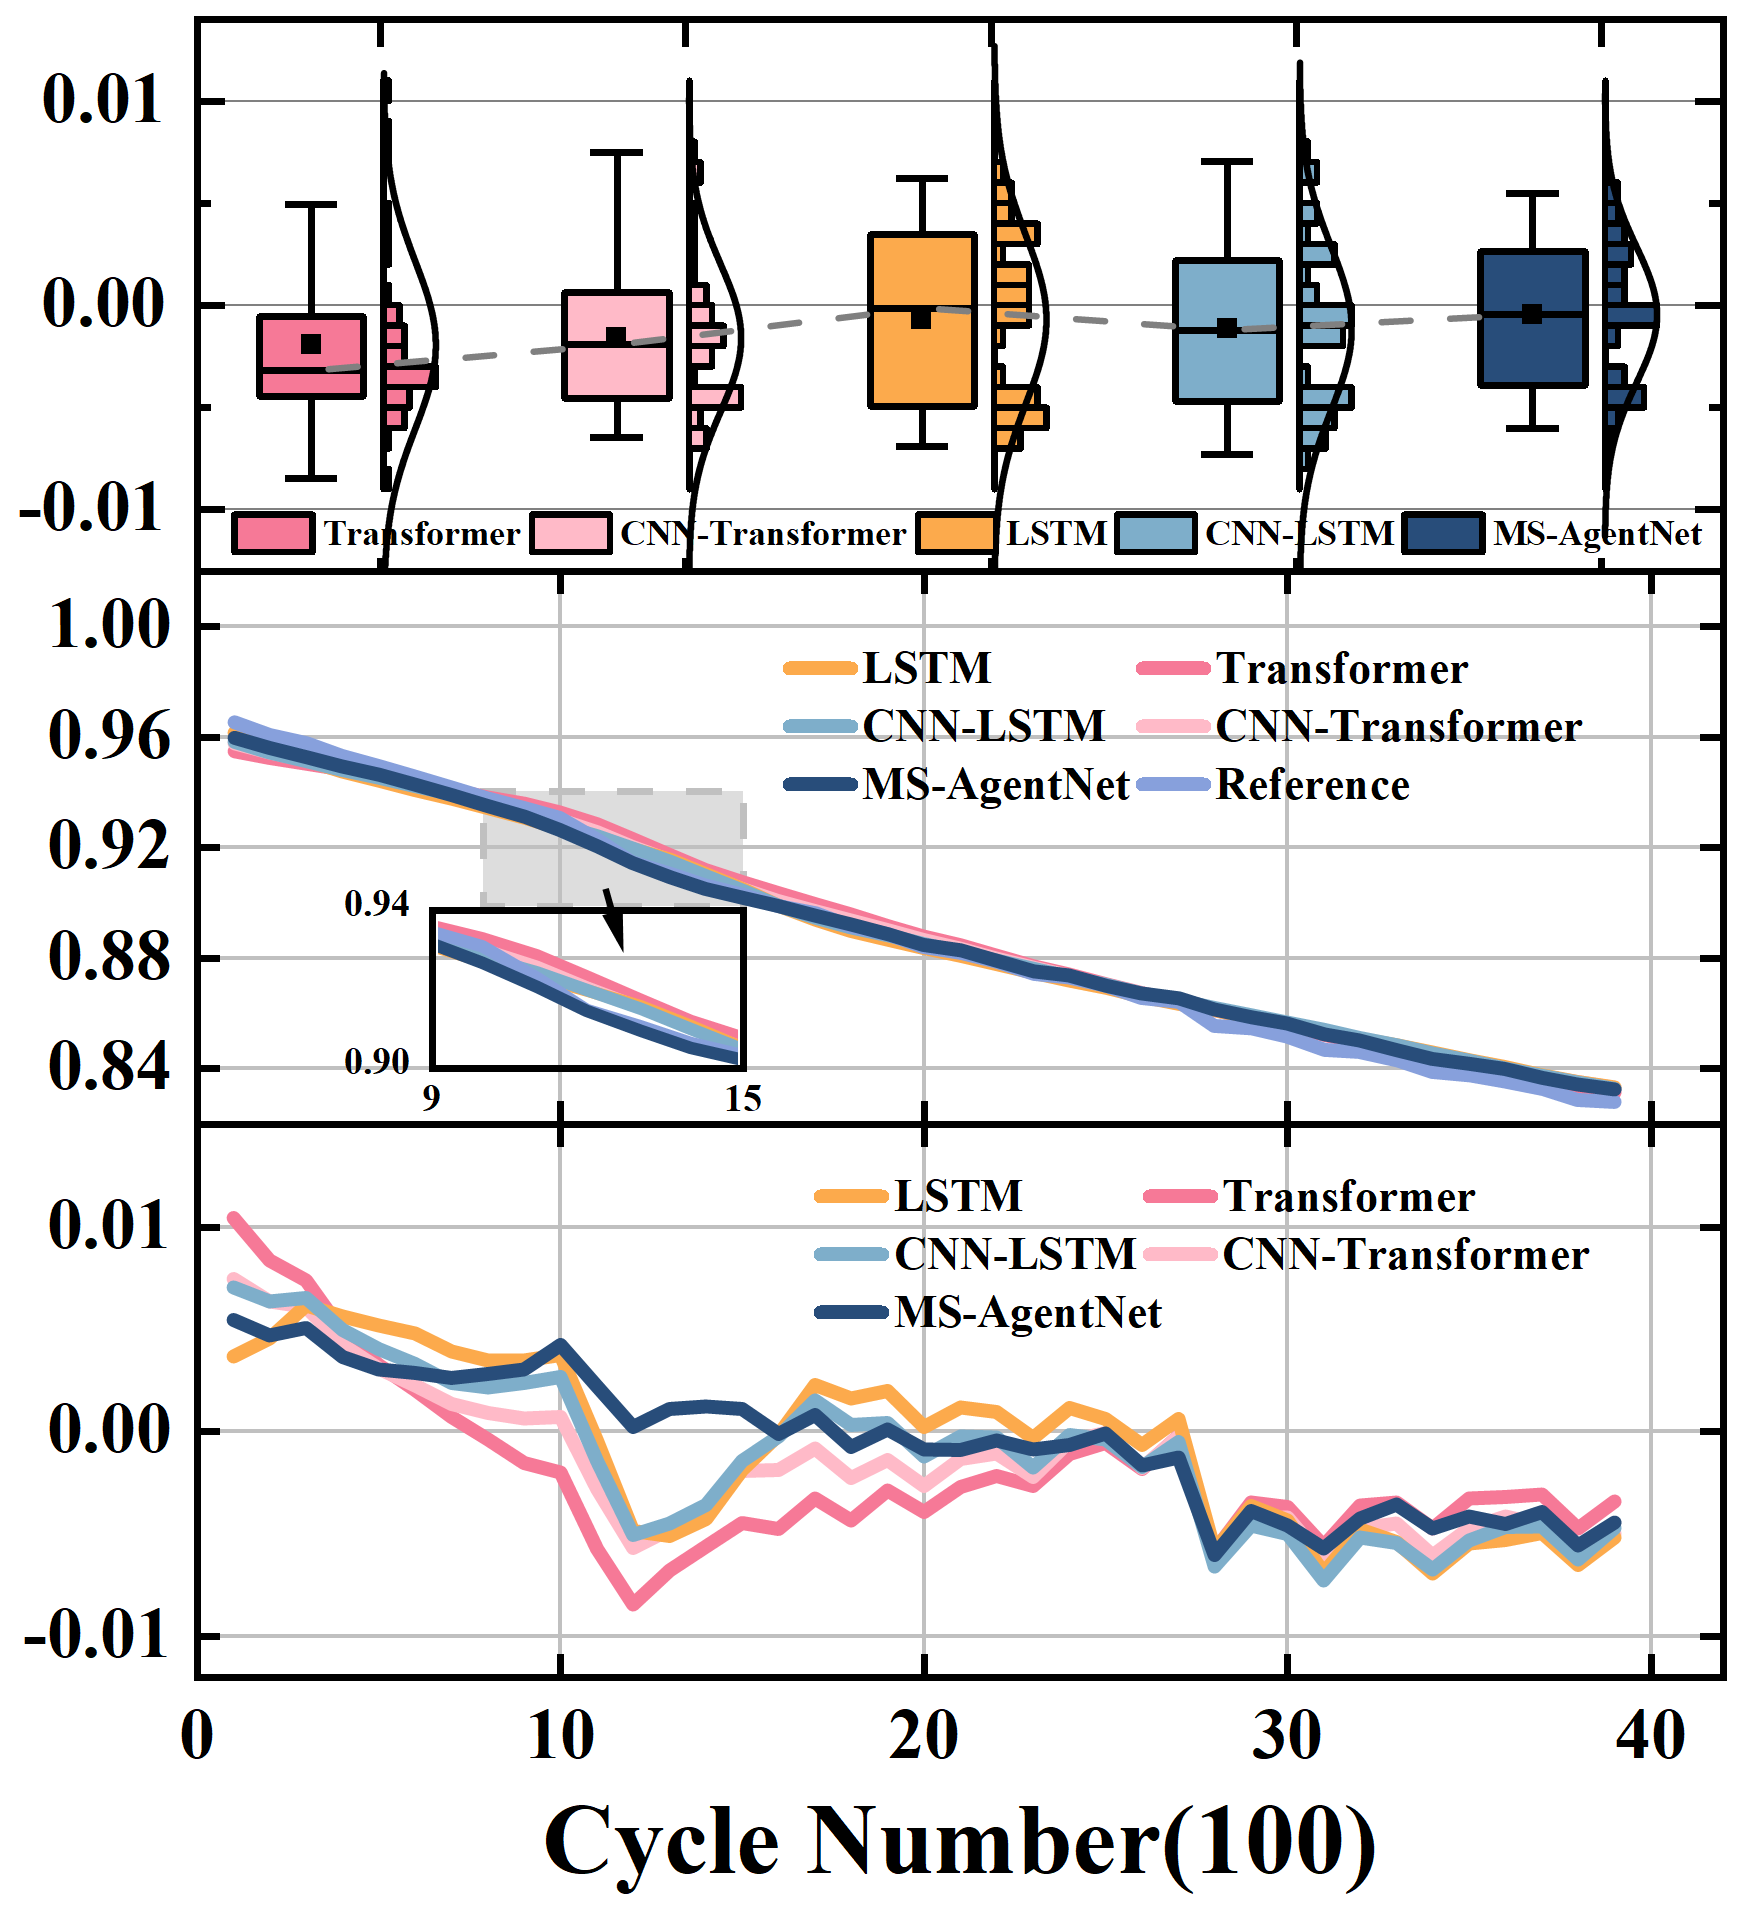
\includegraphics[width=\linewidth]{figures/Oxford/cell5.png}
\end{minipage}%
\hspace{0.01\textwidth}%
\begin{minipage}[t]{0.326\textwidth}\centering
{\fontsize{10}{12}\selectfont\bfseries Cell6}\\[-0.1em]
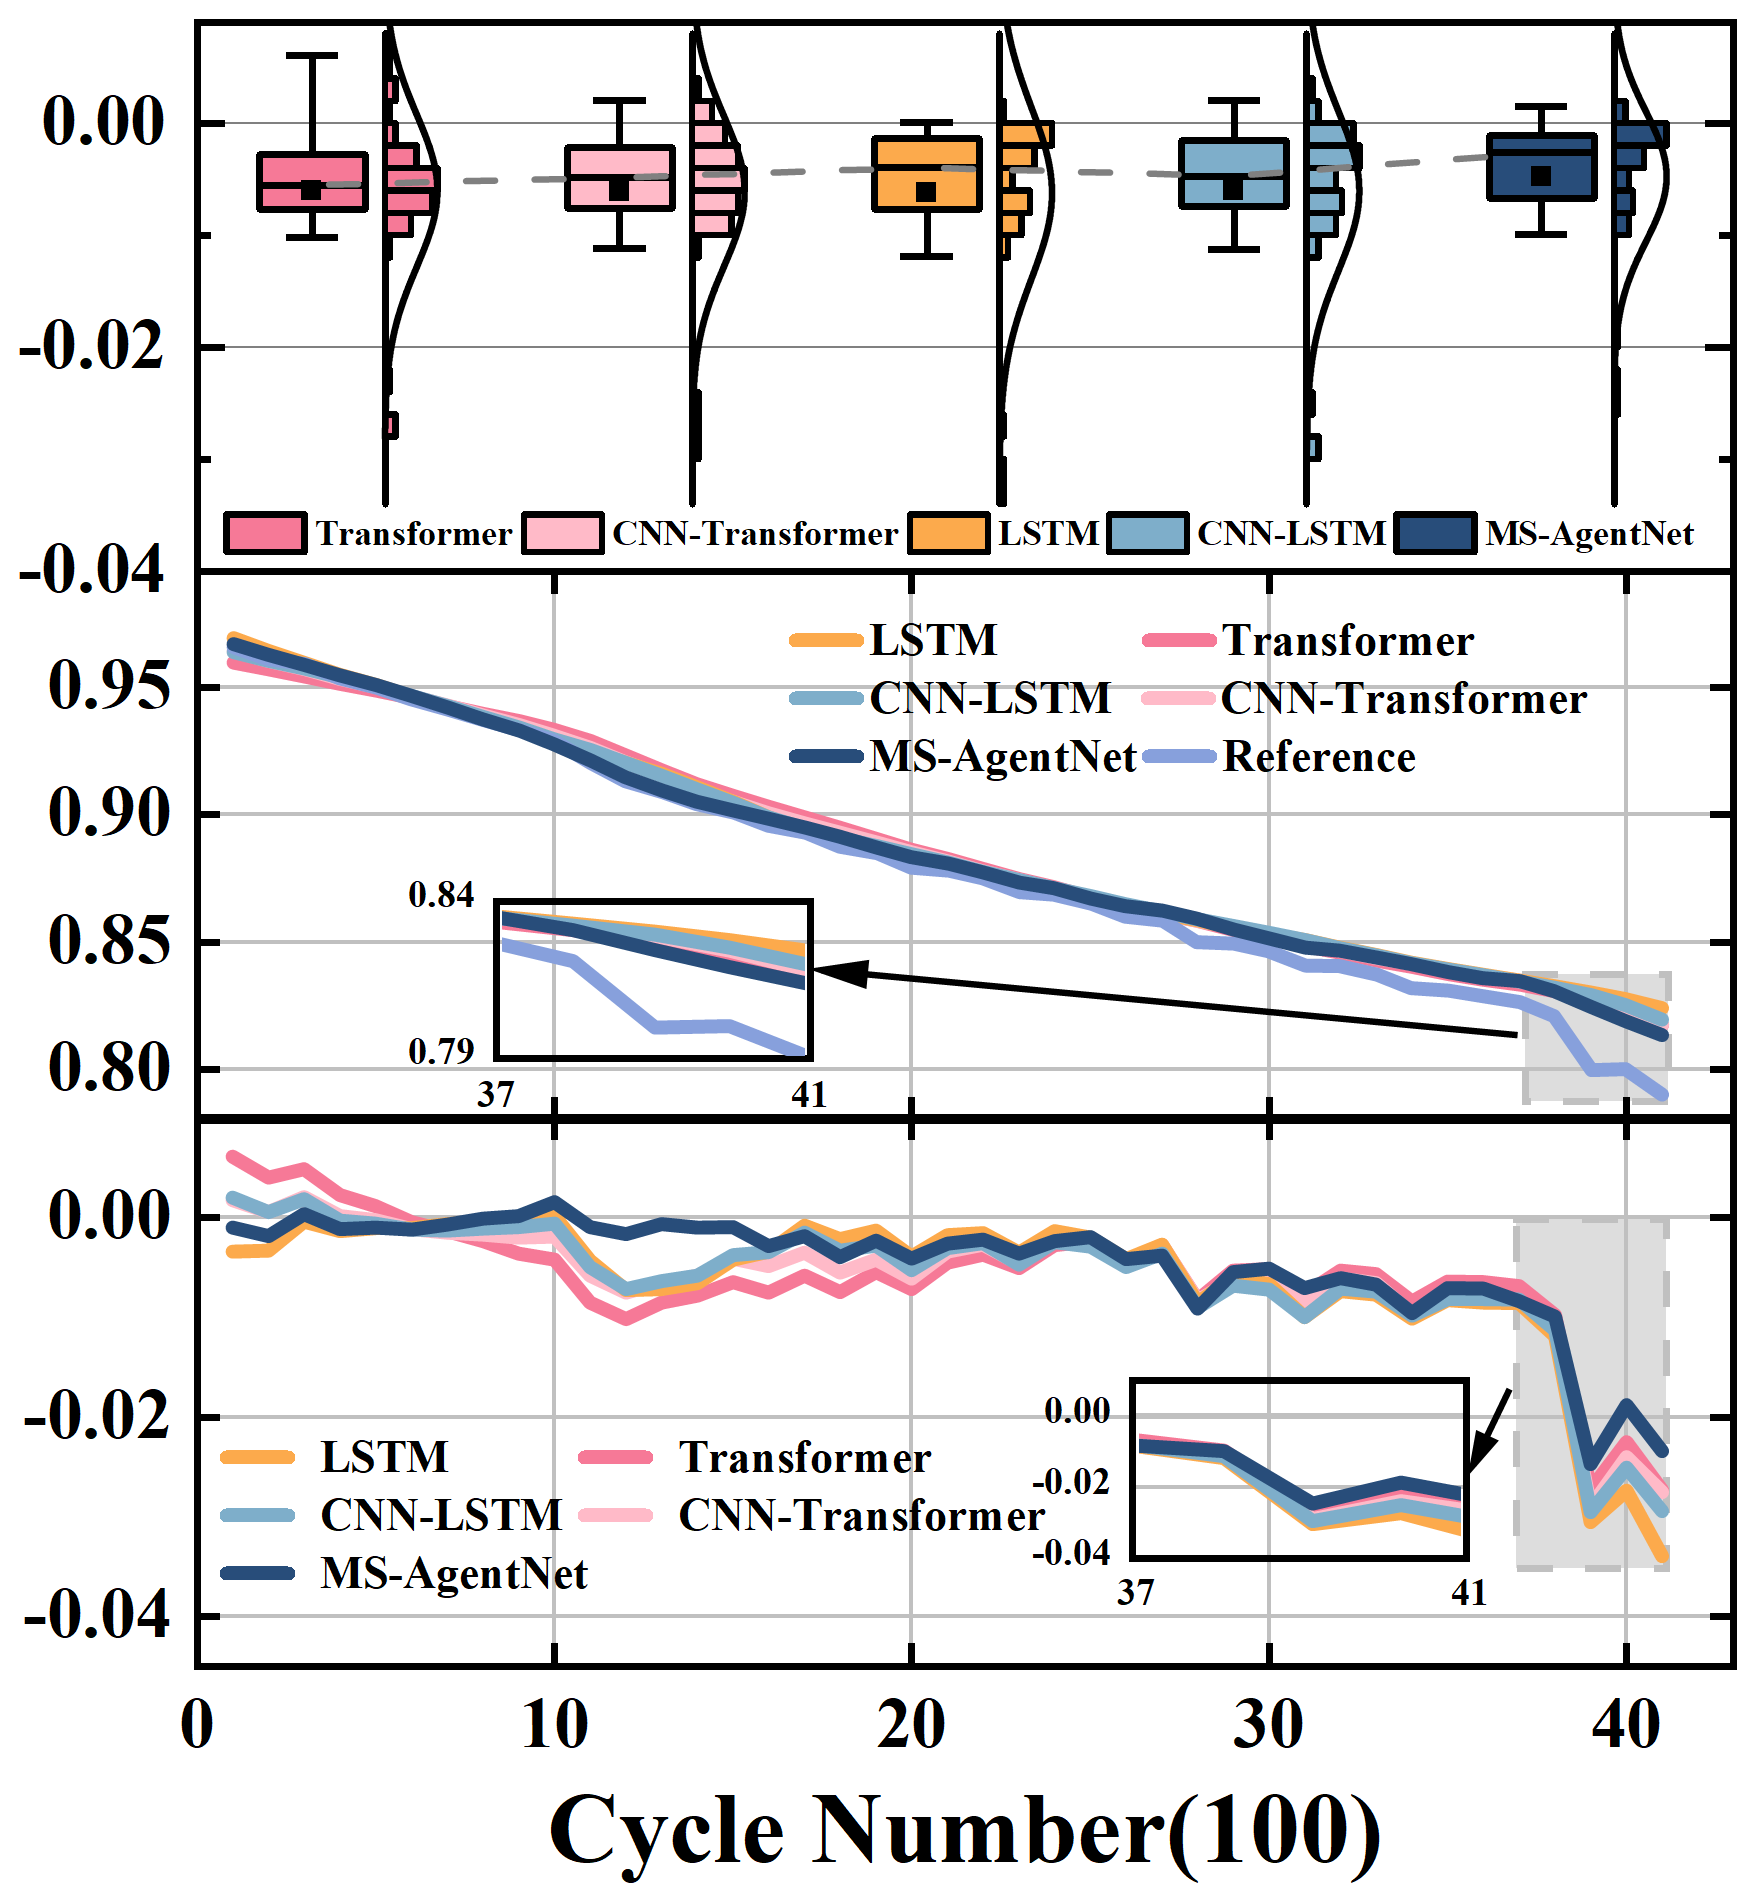
\includegraphics[width=\linewidth]{figures/Oxford/cell6.png}
\end{minipage}%
\\[0.7em]
\begin{minipage}[t]{0.326\textwidth}\centering
{\fontsize{10}{12}\selectfont\bfseries Cell7}\\[-0.1em]
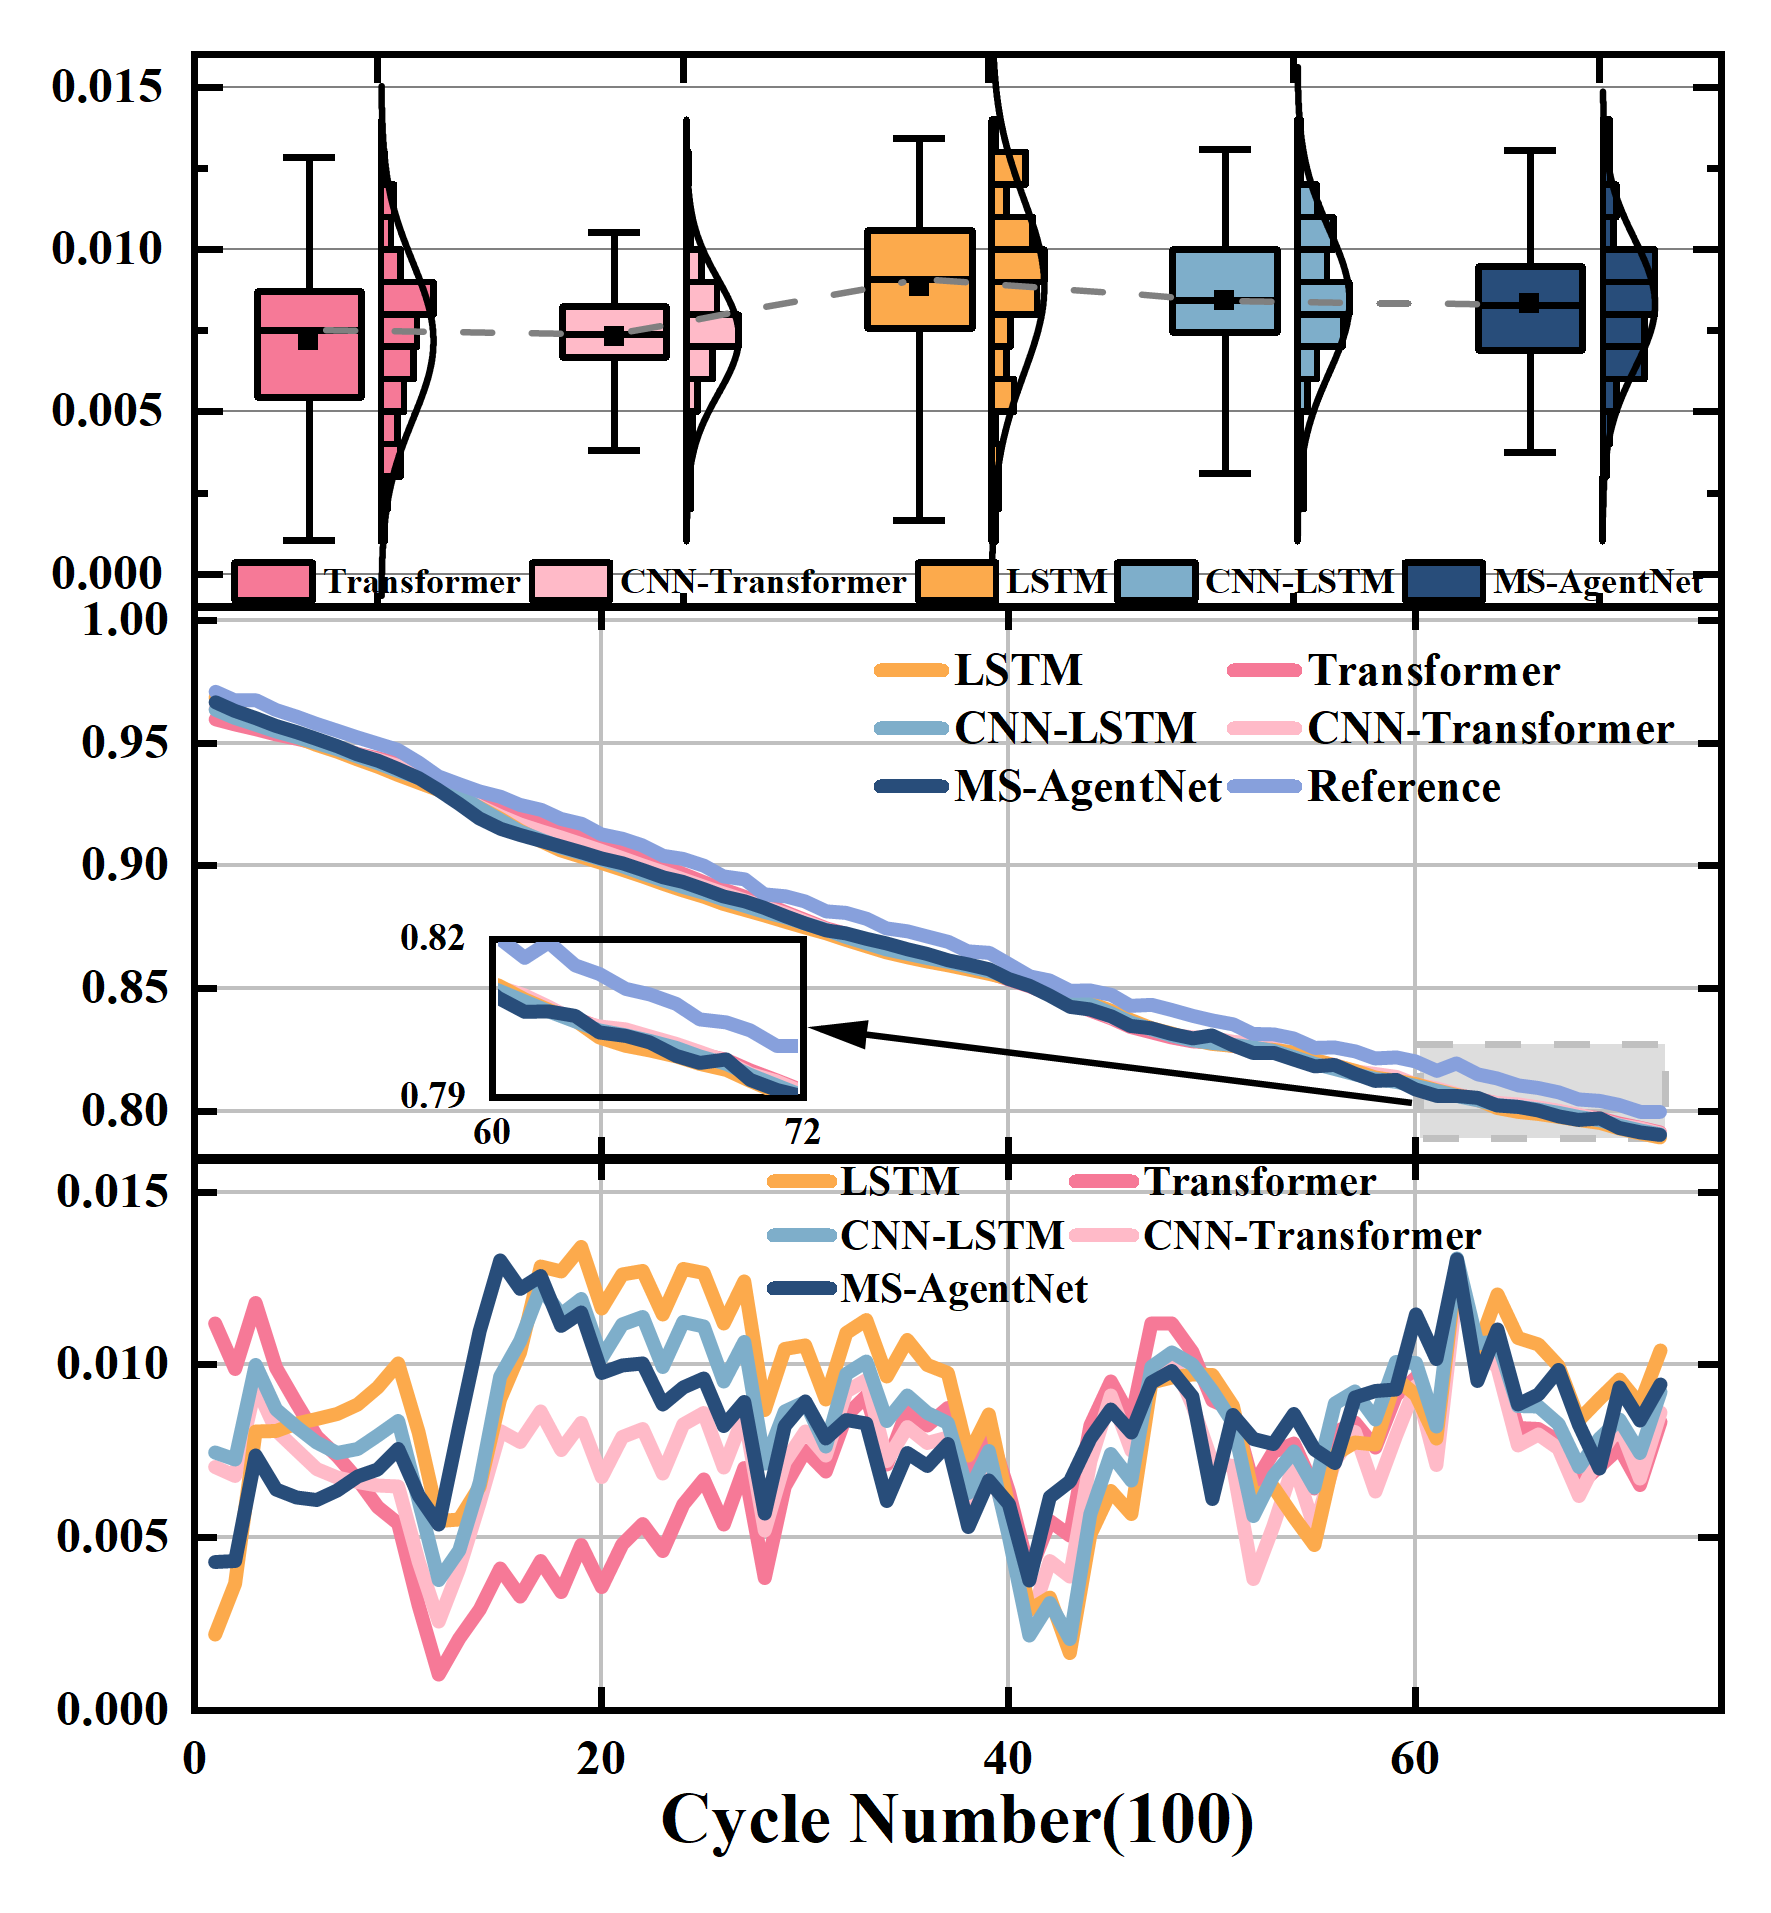
\includegraphics[width=\linewidth]{figures/Oxford/cell7.png}
\end{minipage}%
\hspace{0.01\textwidth}%
\begin{minipage}[t]{0.326\textwidth}\centering
{\fontsize{10}{12}\selectfont\bfseries Cell8}\\[-0.1em]
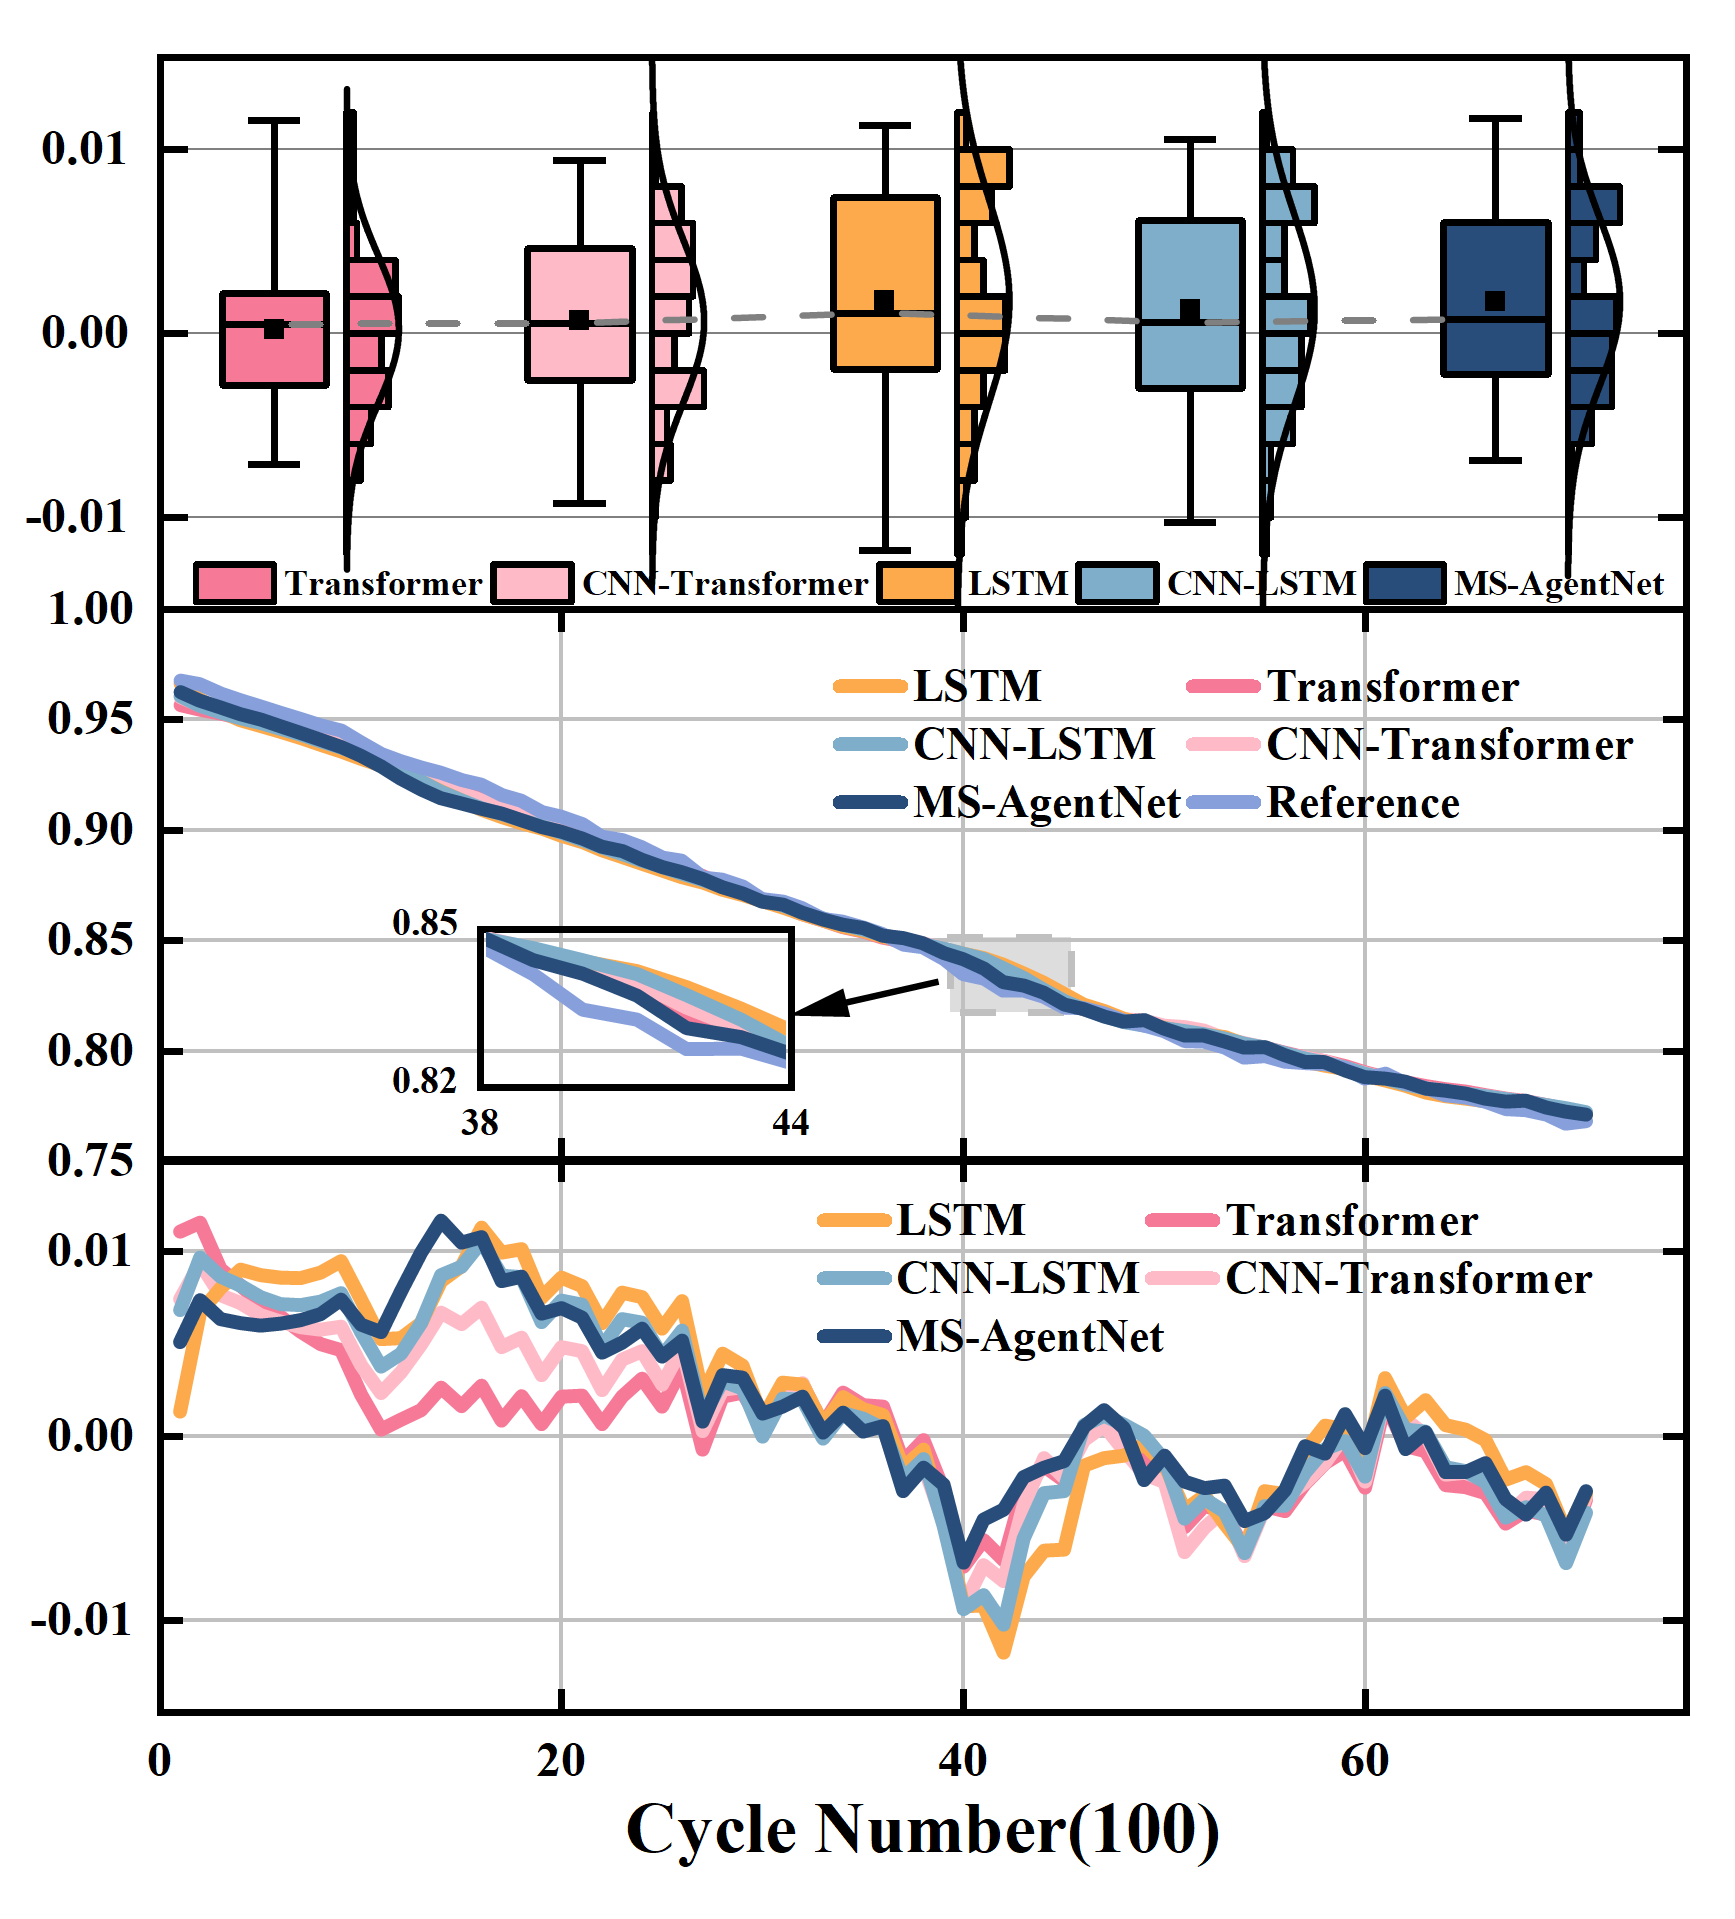
\includegraphics[width=\linewidth]{figures/Oxford/cell8.png}
\end{minipage}%
\end{minipage}%
}
\caption{SOH estimation results of different models on the Oxford dataset.}
\label{fig:4-2}
\end{figure}


总体而言，各模型均能够跟踪电池的容量衰减趋势，但在局部变化区间的预测结果上存在差异。值得注意的是，Cell4 的局部偏离和 Cell6 后段的快速下降使各模型表现出不同程度的跟踪偏差。局部放大结果显示，MS-AgentNet 在上述变化区间仍能较好地跟踪真实 SOH。对于退化轨迹相对平滑的 Cell3 和 Cell5，其预测结果也与真实 SOH 保持较好的贴合。

定量结果表明，MS-AgentNet 在 Cell2、Cell3、Cell5 和 Cell6 上的 $R^2$、MAE、MAPE 和 RMSE 均为最优，并在 Cell4 上取得最高的 $R^2$ 和最低的 RMSE。从 Cell2--Cell8 的平均结果来看，MS-AgentNet 的平均 $R^2$ 为 0.98379，平均 MAE、MAPE 和 RMSE 分别为 0.00524、0.00615 和 0.00638，均在五种模型中排名第一。与 CNN-Transformer、CNN-LSTM、Transformer 和 LSTM 相比，其平均 MAE 分别降低了 2.42\%、8.87\%、4.20\% 和 12.52\%，平均 MAPE 分别降低了 2.38\%、8.48\%、3.76\% 和 12.52\%，平均 RMSE 分别降低了 5.06\%、11.39\%、5.62\% 和 15.83\%。上述结果表明，MS-AgentNet 在 Oxford 数据集上具有较高的 SOH 估计精度和良好的预测鲁棒性。

\begingroup
\TableStyle
\renewcommand{\arraystretch}{0.98}
\setlength\LTleft{0pt plus 1fill}
\setlength\LTright{0pt plus 1fill}
\begin{longtable}{@{}p{16mm}p{41mm}>{\centering\arraybackslash}p{23mm}>{\centering\arraybackslash}p{23mm}>{\centering\arraybackslash}p{23mm}>{\centering\arraybackslash}p{23mm}@{}}
\caption{SOH estimation errors of different models on the Oxford dataset.}\label{tab:4-5}\\
\toprule
Cell & Method & $R^2$ & MAE & MAPE & RMSE \\
\midrule
\endfirsthead
\multicolumn{6}{@{}l}{\fontsize{8.5pt}{11pt}\selectfont Table~\thetable\ continued}\\
\toprule
Cell & Method & $R^2$ & MAE & MAPE & RMSE \\
\midrule
\endhead
\midrule
\multicolumn{6}{r}{\fontsize{8pt}{10pt}\selectfont Continued on next page}\\
\endfoot
\bottomrule
\endlastfoot
Cell2$^{*}$  & MS-AgentNet       & \textbf{0.98890} & \textbf{0.00437} & \textbf{0.00535} & \textbf{0.00706} \\
             & CNN-Transformer  & 0.98532          & 0.00497          & 0.00609          & 0.00812          \\
             & CNN-LSTM         & 0.98341          & 0.00521          & 0.00635          & 0.00863          \\
             & Transformer      & 0.98571          & 0.00512          & 0.00622          & 0.00800          \\
             & LSTM             & 0.97880          & 0.00590          & 0.00725          & 0.00977          \\
\TableGroupSpace
Cell3   & MS-AgentNet       & \textbf{0.99638} & \textbf{0.00295} & \textbf{0.00351} & \textbf{0.00366} \\
        & CNN-Transformer   & 0.99523          & 0.00335          & 0.00396          & 0.00420          \\
        & CNN-LSTM          & 0.99501          & 0.00343          & 0.00404          & 0.00429          \\
        & Transformer       & 0.99472          & 0.00362          & 0.00423          & 0.00440          \\
        & LSTM              & 0.99529          & 0.00327          & 0.00390          & 0.00418          \\
\TableGroupSpace
Cell4   & MS-AgentNet       & \textbf{0.97052} & 0.00838          & 0.00988          & \textbf{0.00898} \\
        & CNN-Transformer   & 0.96942          & \textbf{0.00819} & 0.00969          & 0.00914          \\
        & CNN-LSTM          & 0.96712          & 0.00871          & 0.01026          & 0.00949          \\
        & Transformer       & 0.96931          & 0.00820          & \textbf{0.00966} & 0.00916          \\
        & LSTM              & 0.96267          & 0.00937          & 0.01103          & 0.01011          \\
\TableGroupSpace
Cell5   & MS-AgentNet       & \textbf{0.99257} & \textbf{0.00314} & \textbf{0.00357} & \textbf{0.00362} \\
        & CNN-Transformer   & 0.99002          & 0.00344          & 0.00389          & 0.00417          \\
        & CNN-LSTM          & 0.98912          & 0.00351          & 0.00397          & 0.00434          \\
        & Transformer       & 0.98727          & 0.00391          & 0.00437          & 0.00468          \\
        & LSTM              & 0.99036          & 0.00355          & 0.00400          & 0.00412          \\
\TableGroupSpace
Cell6   & MS-AgentNet       & \textbf{0.96832} & \textbf{0.00619} & \textbf{0.00733} & \textbf{0.00860} \\
        & CNN-Transformer   & 0.96442          & 0.00646          & 0.00764          & 0.00911          \\
        & CNN-LSTM          & 0.96226          & 0.00650          & 0.00771          & 0.00939          \\
        & Transformer       & 0.96402          & 0.00696          & 0.00815          & 0.00917          \\
        & LSTM              & 0.95868          & 0.00626          & 0.00747          & 0.00983          \\
\TableGroupSpace
Cell7   & MS-AgentNet       & 0.97566          & 0.00777          & 0.00894          & 0.00804          \\
        & CNN-Transformer   & \textbf{0.97781} & 0.00731          & 0.00841          & \textbf{0.00766} \\
        & CNN-LSTM          & 0.97081          & 0.00841          & 0.00964          & 0.00880          \\
        & Transformer       & 0.97750          & \textbf{0.00719} & \textbf{0.00830} & 0.00769          \\
        & LSTM              & 0.96768          & 0.00886          & 0.01016          & 0.00926          \\
\TableGroupSpace
Cell8   & MS-AgentNet       & 0.99419          & 0.00389          & 0.00445          & 0.00469          \\
        & CNN-Transformer   & 0.99434          & 0.00384          & 0.00442          & 0.00462          \\
        & CNN-LSTM          & 0.99207          & 0.00445          & 0.00508          & 0.00548          \\
        & Transformer       & \textbf{0.99528} & \textbf{0.00326} & \textbf{0.00377} & \textbf{0.00422} \\
        & LSTM              & 0.99115          & 0.00474          & 0.00539          & 0.00579          \\
\TableGroupSpace
Average & MS-AgentNet       & \textbf{0.98379} & \textbf{0.00524} & \textbf{0.00615} & \textbf{0.00638} \\
        & CNN-Transformer   & 0.98237          & 0.00537          & 0.00630          & 0.00672          \\
        & CNN-LSTM          & 0.97997          & 0.00575          & 0.00672          & 0.00720          \\
        & Transformer       & 0.98197          & 0.00547          & 0.00639          & 0.00676          \\
        & LSTM              & 0.97780          & 0.00599          & 0.00703          & 0.00758          \\
\end{longtable}
\TableNote{Note: Cell2$^{*}$ denotes the cell used for model configuration, and its values are averages of five independent runs. The best results are shown in bold.}
\endgroup

\FloatBarrier

\subsubsection{CALCE和MIT数据集上的跨电池泛化分析}

本节进一步比较了 MS-AgentNet 与四种基线模型在 CALCE CS2、CALCE CX2 和 MIT/Severson 数据集上的 SOH 估计性能。上述数据集在电池材料和充放电协议方面与 Oxford 数据集存在差异，并呈现出平滑衰减、阶段性转折和寿命后期加速衰减等多样化退化动态。各模型的 SOH 估计结果如\cref{fig:4-3}所示。

从整体结果来看，各模型均能够跟踪不同电池的容量衰减趋势，但在局部非线性转折和寿命后期加速衰减阶段的预测表现上存在差异。其中，CX2\_38 经历了多次阶段性转折，并呈现出明显的非线性衰减尾部。局部放大结果显示，进入加速衰减阶段后，各模型的预测偏差逐渐扩大，MS-AgentNet 仍能较好地跟踪其加速衰减轨迹。对于退化轨迹较为连续的 CS2\_38 和 b3c29，MS-AgentNet 也能够保持与真实 SOH 的较好贴合。

\Cref{tab:4-6}列出了各模型在六节电池上的 SOH 估计误差。MS-AgentNet 在其中五节电池上的 $R^2$、MAE、MAPE 和 RMSE 均为最优。值得注意的是，在具有阶段性转折和非线性衰减尾部的 CX2\_38 上，MS-AgentNet 的 MAPE 仅为 0.037673，较 CNN-Transformer 和 Transformer 分别降低了 59.75\% 和 51.80\%，表明模型在寿命后期加速衰减阶段仍能保持较低的预测误差。

从六节电池的平均结果来看，MS-AgentNet 的平均 $R^2$ 为 0.9896，平均 MAE、MAPE 和 RMSE 分别为 0.00707、0.013335 和 0.01188，均在五种模型中排名第一。与 CNN-Transformer、CNN-LSTM、Transformer 和 LSTM 相比，其平均 MAE 分别降低了 13.50\%、26.02\%、9.11\% 和 22.94\%，平均 MAPE 分别降低了 42.19\%、60.08\%、34.49\% 和 58.17\%，平均 RMSE 分别降低了 12.04\%、26.52\%、7.97\% 和 23.09\%。综合不同退化场景，MS-AgentNet 在平滑衰减、阶段性转折和寿命后期加速衰减过程中均保持了较低的估计误差，体现出较好的预测鲁棒性和跨电池泛化能力。

% Shared physical geometry for Fig. 8 and Fig. 9.
% Every cell: 62 x 70 mm; axes frame: 48 x 54 mm at (13.5, 9).
% Titles are centered on the axes at x = 37.5 mm, not on label padding.
% Per-image transforms preserve all source annotations and equalize frame size.
\providecommand{\ComparisonPanel}[6]{%
  \begingroup\setlength{\unitlength}{1mm}%
  \begin{picture}(62,70)%
    \put(#3,#4){\includegraphics[width=#5mm,height=#6mm]{#2}}%
    \put(37.5,67){\makebox(0,0){\fontsize{10pt}{12pt}\selectfont\bfseries\strut #1}}%
  \end{picture}%
  \endgroup
}

\begin{figure}[!htb]
\centering
\makebox[\textwidth][c]{%
\begin{minipage}{190mm}\centering
\ComparisonPanel{CS2\_37}{figures/CSCXMIT/CS-37.png}{0.55160}{1.49007}{61.51274}{63.49308}%
\hspace{2mm}%
\ComparisonPanel{CX2\_37}{figures/CSCXMIT/CX-37.png}{7.42564}{1.68784}{54.57534}{61.95926}%
\hspace{2mm}%
\ComparisonPanel{b3c13}{figures/CSCXMIT/b3c13.png}{7.42167}{1.67467}{54.51697}{61.87635}%
\\[2mm]
\ComparisonPanel{CS2\_38}{figures/CSCXMIT/CS-38.png}{1.57045}{1.72202}{60.39922}{62.35018}%
\hspace{2mm}%
\ComparisonPanel{CX2\_38}{figures/CSCXMIT/CX-38.png}{7.42564}{1.66587}{56.42270}{62.66466}%
\hspace{2mm}%
\ComparisonPanel{b3c29}{figures/CSCXMIT/b3c29.png}{7.42167}{1.81726}{54.51697}{61.82984}%
\end{minipage}%
}
\caption{SOH estimation results of different models on the CALCE and MIT/Severson datasets.}
\label{fig:4-3}
\end{figure}

\begin{table}[!htbp]
\caption{SOH estimation errors of different models on the CALCE and MIT/Severson datasets.}
\label{tab:4-6}
\centering
\zihao{-5}
\setlength{\tabcolsep}{2.2pt}
\renewcommand{\arraystretch}{1.02}
\begin{ThreePartTable}
\begin{tabularx}{0.98\linewidth}{>{\raggedright\arraybackslash}p{0.21\linewidth}>{\raggedright\arraybackslash}p{0.24\linewidth}>{\centering\arraybackslash}p{0.10\linewidth}>{\centering\arraybackslash}p{0.10\linewidth}>{\centering\arraybackslash}p{0.14\linewidth}>{\centering\arraybackslash}p{0.10\linewidth}}
\toprule
Dataset & Method & $R^2$ & MAE & MAPE & RMSE \\
\midrule
\makecell[l]{CALCE CS2\\(CS2\_38)} & MS-AgentNet       & \textbf{0.9798} & \textbf{0.0120} & \textbf{0.015984} & \textbf{0.0174} \\
                                  & CNN-Transformer   & 0.9779          & 0.0126          & 0.016928          & 0.0182          \\
                                  & CNN-LSTM          & 0.9778          & 0.0125          & 0.016680          & 0.0183          \\
                                  & Transformer       & 0.9787          & 0.0122          & 0.016434          & 0.0179          \\
                                  & LSTM              & 0.9776          & 0.0128          & 0.017085          & 0.0184          \\
\addlinespace[0.5pt]
\makecell[l]{CALCE CX2\\(CX2\_38)} & MS-AgentNet       & \textbf{0.9947} & \textbf{0.0106} & \textbf{0.037673} & \textbf{0.0193} \\
                                  & CNN-Transformer   & 0.9895          & 0.0154          & 0.093595          & 0.0269          \\
                                  & CNN-LSTM          & 0.9785          & 0.0207          & 0.152435         & 0.0387          \\
                                  & Transformer       & 0.9916          & 0.0138          & 0.078160          & 0.0243          \\
                                  & LSTM              & 0.9804          & 0.0201          & 0.145055         & 0.0370          \\
\addlinespace[0.5pt]
\makecell[l]{MIT/Severson\\(b3c29)} & MS-AgentNet      & \textbf{0.9972} & \textbf{0.0018} & \textbf{0.001960} & \textbf{0.0022} \\
                                   & CNN-Transformer  & 0.9960          & 0.0021          & 0.002302          & 0.0025          \\
                                   & CNN-LSTM         & 0.9879          & 0.0035          & 0.003808          & 0.0044          \\
                                   & Transformer      & 0.9971          & 0.0018          & 0.001976          & 0.0022          \\
                                   & LSTM             & 0.9952          & 0.0025          & 0.002667          & 0.0028          \\
\addlinespace[1pt]
Average                           & MS-AgentNet       & \textbf{0.9906} & \textbf{0.0081} & \textbf{0.018539} & \textbf{0.0129} \\
                                  & CNN-Transformer   & 0.9878          & 0.0100          & 0.037608          & 0.0159          \\
                                  & CNN-LSTM          & 0.9814          & 0.0122          & 0.057641          & 0.0204          \\
                                  & Transformer       & 0.9891          & 0.0093          & 0.032190          & 0.0148          \\
                                  & LSTM              & 0.9844          & 0.0118          & 0.054936          & 0.0194          \\
\bottomrule
\end{tabularx}
\begin{tablenotes}[flushleft]
\footnotesize
\item[] \parbox[t]{0.98\linewidth}{Note: Results are averaged over five independent runs. Average denotes the macro-average over the three independent evaluation cells. The best results are determined using unrounded values and are shown in bold.}
\end{tablenotes}
\end{ThreePartTable}
\end{table}

\FloatBarrier

\subsection{跨数据集迁移实验}

当源域与目标域来自不同数据集时，化学体系、运行协议和退化轨迹差异可能引起域偏移\cite{ref52,ref59}。为评价 MS-AgentNet 的跨数据集迁移能力，本文设置源域直接测试和少样本适应两类实验。源域直接测试（source-only）仅利用源域参考电池训练模型，并在不使用目标域数据更新参数的情况下直接测试目标域电池；少样本适应则固定特征提取模块，利用目标域参考电池前 30\% 的循环数据更新读出层，再在目标域测试电池上进行评价\cite{ref52,ref58}。

CALCE CS2、CALCE CX2 和 Oxford 分别视为三个数据域，其中 CS2\_36、CX2\_36 和 Oxford Cell1 用于源域训练或目标域适应，CS2\_38、CX2\_38 和 Oxford Cell3 仅用于目标域测试。CALCE CS2 与 CALCE CX2 均属于 LCO 化学体系，Oxford 采用 NCO-LCO 混合化学体系，因此实验同时覆盖同化学体系和跨化学体系迁移。为保持源域与目标域的输入定义一致，各迁移方向统一采用 $CCCT(3.8,\allowbreak 4.0)$ 和 $Q_{\mathrm{dch}}(3.8,\allowbreak 3.4)/C_{\mathrm{rated}}$ 两项健康指标。

\subsubsection{不同迁移方向的性能比较}

如\cref{tab:4-7}所示，CS2→CX2 和 CX2→CS2 的 $R^2$ 分别为 0.8421 和 0.7847，MAE 分别为 0.0697 和 0.0388，表明模型在两个 CALCE 数据域之间仍能较好地表征退化趋势。相比之下，四个涉及 Oxford 的迁移方向的 MAE 为 0.1530～0.6346，且 $R^2$ 均低于 0，显示直接迁移性能随数据域组合和迁移方向发生明显变化。

少样本适应结果见\cref{tab:4-8}。适应后，六个迁移方向的 MAE、MAPE 和 RMSE 均有所降低。以 MAE 为例，两个 CALCE 数据域之间的降幅为 21.91\%～45.91\%，CALCE→Oxford 方向的降幅为 86.84\%～87.61\%，Oxford→CALCE 方向的降幅为 13.27\%～31.21\%。从 $R^2$ 看，适应后的 CS2→CX2 和 CX2→CS2 分别达到 0.9566 和 0.8806，而四个涉及 Oxford 的迁移方向仍低于 0，表明涉及 Oxford 的跨数据集迁移较两个 CALCE 数据域之间的迁移更具挑战性。

\begin{table}
\TableStyle
\caption{Direct cross-dataset transfer results.}
\label{tab:4-7}
\begin{tabularx}{\linewidth}{@{\extracolsep{\fill}}L{0.90}L{0.90}C{1.20}C{1.00}C{1.00}C{1.00}@{}}
\toprule
Source & Target & $R^2$ & MAE & MAPE & RMSE \\
\midrule
CS2 & CX2 & $0.8421$ & $0.0697$ & $0.3974$ & $0.1051$ \\
CS2 & Oxford & $-60.5701$ & $0.4761$ & $0.5573$ & $0.4778$ \\
CX2 & CS2 & $0.7847$ & $0.0388$ & $0.0557$ & $0.0568$ \\
CX2 & Oxford & $-108.6169$ & $0.6346$ & $0.7423$ & $0.6375$ \\
Oxford & CS2 & $-1.5309$ & $0.1530$ & $0.2196$ & $0.1950$ \\
Oxford & CX2 & $-1.4786$ & $0.3528$ & $1.5040$ & $0.4164$ \\
\bottomrule
\end{tabularx}
\end{table}

\begin{table}[!htbp]
\caption{Transfer results after 30\% target-domain adaptation.}
\label{tab:4-8}
\centering
\zihao{-5}
\setlength{\tabcolsep}{3.0pt}
\renewcommand{\arraystretch}{1.05}
\begin{ThreePartTable}
\begin{tabularx}{0.90\linewidth}{>{\raggedright\arraybackslash}p{0.25\linewidth}>{\centering\arraybackslash}p{0.13\linewidth}>{\centering\arraybackslash}p{0.12\linewidth}>{\centering\arraybackslash}p{0.12\linewidth}>{\centering\arraybackslash}p{0.12\linewidth}}
\toprule
\makecell[l]{Source domain\\(training cell)} & Metric & CS2 & CX2 & Oxford \\
\midrule
\makecell[l]{CALCE CS2\\(CS2\_36)} & $R^2$      & ---    & 0.9566   & -0.2679 \\
                      & MAE        & ---    & 0.0377   & 0.0590  \\
                      & MAPE       & ---    & 0.1830   & 0.0722  \\
                      & RMSE       & ---    & 0.0533   & 0.0685  \\
\addlinespace[1pt]
\makecell[l]{CALCE CX2\\(CX2\_36)} & $R^2$      & 0.8806 & ---      & -1.6085 \\
                      & MAE        & 0.0303 & ---      & 0.0835  \\
                      & MAPE       & 0.0406 & ---      & 0.1024  \\
                      & RMSE       & 0.0422 & ---      & 0.0982  \\
\addlinespace[1pt]
\makecell[l]{Oxford\\(Cell1)} & $R^2$     & -1.1030 & -0.4809 & ---     \\
                     & MAE       & 0.1327  & 0.2427  & ---     \\
                     & MAPE      & 0.1935  & 1.2100  & ---     \\
                     & RMSE      & 0.1777  & 0.3218  & ---     \\
\bottomrule
\end{tabularx}
\begin{tablenotes}[flushleft]
\footnotesize
\item[] \parbox[t]{0.98\linewidth}{Note: Results are averaged over three independent runs.}
\end{tablenotes}
\end{ThreePartTable}
\end{table}


\subsubsection{目标域适配比例的影响}

分别以 CS2\_36 和 CX2\_36 作为源域，使用 Oxford Cell1 的前置循环数据进行读出层适配，并将适配比例依次设置为 10\%、30\%、50\% 和 70\%，结果见\cref{tab:4-9}。


随着适配比例由 10\% 增至 70\%，两种源域设置下的 MAE、MAPE 和 RMSE 均持续下降。以 CS2 为源域时，MAE 由 0.0831 降至 0.0252，$R^2$ 由 -1.3934 提高至 0.7650，并在 50\% 适配比例下由负转正；以 CX2 为源域时，MAE 由 0.1095 降至 0.0559，$R^2$ 由 -3.2217 提高至 70\% 适配比例下的 -0.1268。四种适配比例下，CS2 源域的 $R^2$ 均高于 CX2 源域的对应结果。

进一步比较相邻适配比例，CS2 和 CX2 源域从 30\% 增至 50\% 时，MAE 分别降低 0.0224 和 0.0221；从 50\% 增至 70\% 时，降幅分别缩小至 0.0114 和 0.0055。结果表明，增加目标域观测能够持续改善模型在 Oxford 数据域上的适配性能；在相同适配比例下，CS2 源域始终取得更低的估计误差和更高的 $R^2$，进一步体现了源域选择对跨数据集适配性能的影响。

\begin{table}[!htbp]
\caption{Transfer results under different adaptation ratios.}
\label{tab:4-9}
\centering
\zihao{-5}
\setlength{\tabcolsep}{2.4pt}
\renewcommand{\arraystretch}{1.04}
\begin{ThreePartTable}
\begin{tabularx}{0.90\linewidth}{>{\raggedright\arraybackslash}p{0.25\linewidth}>{\centering\arraybackslash}p{0.13\linewidth}>{\centering\arraybackslash}p{0.10\linewidth}>{\centering\arraybackslash}p{0.10\linewidth}>{\centering\arraybackslash}p{0.10\linewidth}>{\centering\arraybackslash}p{0.10\linewidth}}
\toprule
\makecell[l]{Source domain\\(training cell)} & Metric & 10\% & 30\% & 50\% & 70\% \\
\midrule
\makecell[l]{CALCE CS2\\(CS2\_36)} & $R^2$      & -1.3934 & -0.2679 & 0.5094 & 0.7650 \\
                      & MAE        & 0.0831  & 0.0590  & 0.0366 & 0.0252 \\
                      & MAPE       & 0.1015  & 0.0722  & 0.0445 & 0.0305 \\
                      & RMSE       & 0.0942  & 0.0685  & 0.0426 & 0.0293 \\
\addlinespace[1pt]
\makecell[l]{CALCE CX2\\(CX2\_36)} & $R^2$      & -3.2217 & -1.6085 & -0.3836 & -0.1268 \\
                      & MAE        & 0.1095  & 0.0835  & 0.0614  & 0.0559 \\
                      & MAPE       & 0.1339  & 0.1024  & 0.0747  & 0.0677 \\
                      & RMSE       & 0.1251  & 0.0982  & 0.0716  & 0.0646 \\
\bottomrule
\end{tabularx}
\begin{tablenotes}[flushleft]
\footnotesize
\item[] \parbox[t]{0.98\linewidth}{Note: Results are averaged over three independent runs.}
\end{tablenotes}
\end{ThreePartTable}
\end{table}

\FloatBarrier


\subsection{模块消融与模型复杂度分析}

为进一步验证 MS-AgentNet 的有效性和效率，在主对比实验基础上开展消融研究与复杂度分析。消融研究通过移除或组合关键模块，考察各模块对预测性能的作用；复杂度分析则从计算量、参数量和存储占用等方面评估模型开销。

\subsubsection{模块消融分析}

高效注意力通过压缩信息交互降低标准注意力的计算开销\cite{ref39,ref40,ref43,ref44}，但这一过程可能削弱局部细粒度退化信息的表达\cite{ref31}；直接叠加标准卷积虽然能够增强局部特征建模，却会增加参数量和计算负担\cite{ref31,ref71}。为兼顾局部信息保留与计算效率，MS-AgentNet 结合多尺度 DSConv 与 RAA，分别完成局部特征提取和跨位置信息交互。为考察两类模块的单独作用及组合效果，消融实验设置 M1–M4 四种变体。其中，M1 仅保留基础骨干网络，M2 在 M1 基础上加入多尺度 DSConv，M3 在 M1 基础上加入 RAA，M4 则同时集成多尺度 DSConv 与 RAA。


如\cref{tab:4-10}所示，与基础模型 M1 相比，加入多尺度 DSConv 后，M2 在 CX2 和 Oxford 数据集上的综合平均误差分别降低约 1.20\% 和 8.45\%；加入 RAA 后，M3 在 CS2、CX2 和 Oxford 数据集上的综合平均误差分别降低约 3.18\%、11.60\% 和 15.49\%。两种模块单独使用时均改善了部分数据集上的估计结果，但未在四个数据集上同时取得更低误差。

当多尺度 DSConv 与 RAA 共同集成后，完整模型 M4 在四个数据集上均取得最低或并列最低的综合平均误差。以 CX2 和 Oxford 数据集为例，其综合平均误差分别由 M1 的 0.0500 和 0.0071 降低至 0.0225 和 0.0059，相对降低 54.94\% 和 16.52\%。在 CS2 数据集上，M3 的 MAE 略低于 M4，而 M4 在 RMSE、MAPE 和综合平均误差上表现更优。总体结果表明，完整模型获得了比单模块变体更稳定的综合表现，体现了多尺度局部特征提取与跨位置信息交互的互补作用。

为进一步区分多尺度 DSConv 中两个卷积尺度的作用，固定 RAA 模块并仅调整卷积尺度，设置 S0（仅保留 RAA）、S5（RAA 与核长度为 5 的 DSConv-S）、S31（RAA 与核长度为 31 的 DSConv-L）和 SFull（RAA、DSConv-S 与 DSConv-L）四种尺度变体。其中，S0 和 SFull 分别与\cref{tab:4-10}中的 M3 和 M4 对应。

\Cref{tab:4-11}的结果显示，单一卷积尺度的收益随数据集而变化。在具有阶段性转折和非线性衰减尾部的 CX2 数据集上，S31 将综合平均误差由 S0 的 0.0442 降至 0.0348，相对降低 21.27\%，这一结果与 DSConv-L 进行长尺度特征细化的设计目标一致。在 MIT 数据集上，S5 相对 S0 降低约 3.85\%；在 CS2 和 Oxford 数据集上，S0 的综合平均误差仍低于两个单尺度变体。当两个卷积尺度共同使用时，SFull 在四个数据集上均取得最低的综合平均误差。与最佳单尺度变体相比，SFull 在 CX2 和 MIT 数据集上的误差分别降低 35.34\% 和 20.00\%。因此，同时保留短核与长核能够取得比单一尺度更一致的综合结果，支持多尺度 DSConv 的结构设计。

\begin{table}[!htbp]
\caption{Ablation results on different datasets.}
\label{tab:4-10}
\centering
\zihao{-5}
\setlength{\tabcolsep}{2.4pt}
\renewcommand{\arraystretch}{1.04}
\begin{ThreePartTable}
\begin{tabularx}{0.98\linewidth}{>{\centering\arraybackslash}p{0.08\linewidth}>{\centering\arraybackslash}p{0.11\linewidth}>{\centering\arraybackslash}p{0.08\linewidth}>{\centering\arraybackslash}p{0.10\linewidth}>{\centering\arraybackslash}p{0.06\linewidth}>{\centering\arraybackslash}p{0.08\linewidth}>{\centering\arraybackslash}p{0.08\linewidth}>{\centering\arraybackslash}p{0.09\linewidth}>{\centering\arraybackslash}p{0.09\linewidth}>{\centering\arraybackslash}p{0.09\linewidth}}
\toprule
Dataset & Model & Backbone & \makecell[c]{Multi-scale\\DSConv} & RAA & MAE & RMSE & MAPE & Average & Reduction \\
\midrule
CS2    & M1                           & \ding{51} & ---        & ---        & 0.0123 & 0.0183 & 0.0166 & 0.0157 & 3.74\%  \\
       & M2                           & \ding{51} & \ding{51}  & ---        & 0.0130 & 0.0184 & 0.0171 & 0.0162 & 6.49\%  \\
       & M3                           & \ding{51} & ---        & \ding{51}  & 0.0119 & 0.0178 & 0.0161 & 0.0152 & 0.62\%  \\
       & \makecell[c]{M4\\(Proposed)} & \ding{51} & \ding{51}  & \ding{51}  & 0.0120 & 0.0174 & 0.0160 & 0.0151 & ---     \\
\addlinespace[1pt]
CX2    & M1                           & \ding{51} & ---        & ---        & 0.0170 & 0.0294 & 0.1035 & 0.0500 & 54.94\% \\
       & M2                           & \ding{51} & \ding{51}  & ---        & 0.0164 & 0.0284 & 0.1033 & 0.0494 & 54.40\% \\
       & M3                           & \ding{51} & ---        & \ding{51}  & 0.0156 & 0.0270 & 0.0899 & 0.0442 & 49.05\% \\
       & \makecell[c]{M4\\(Proposed)} & \ding{51} & \ding{51}  & \ding{51}  & 0.0106 & 0.0193 & 0.0377 & 0.0225 & ---     \\
\addlinespace[1pt]
MIT    & M1                           & \ding{51} & ---        & ---        & 0.0019 & 0.0022 & 0.0020 & 0.0020 & 2.43\%  \\
       & M2                           & \ding{51} & \ding{51}  & ---        & 0.0021 & 0.0025 & 0.0023 & 0.0023 & 14.16\% \\
       & M3                           & \ding{51} & ---        & \ding{51}  & 0.0024 & 0.0028 & 0.0026 & 0.0026 & 23.91\% \\
       & \makecell[c]{M4\\(Proposed)} & \ding{51} & \ding{51}  & \ding{51}  & 0.0018 & 0.0022 & 0.0020 & 0.0020 & ---     \\
\addlinespace[1pt]
Oxford & M1                           & \ding{51} & ---        & ---        & 0.0063 & 0.0076 & 0.0073 & 0.0071 & 16.52\% \\
       & M2                           & \ding{51} & \ding{51}  & ---        & 0.0058 & 0.0070 & 0.0067 & 0.0065 & 9.50\%  \\
       & M3                           & \ding{51} & ---        & \ding{51}  & 0.0054 & 0.0063 & 0.0062 & 0.0060 & 1.52\%  \\
       & \makecell[c]{M4\\(Proposed)} & \ding{51} & \ding{51}  & \ding{51}  & 0.0053 & 0.0062 & 0.0062 & 0.0059 & ---     \\
\bottomrule
\end{tabularx}
\end{ThreePartTable}
\end{table}

\begin{table}[H]
\TableStyle
\caption{Effects of different convolution scales.}
\label{tab:4-11}
\begin{tabularx}{\linewidth}{@{\extracolsep{\fill}}L{0.90}C{0.90}C{0.75}C{0.75}C{0.60}C{1.275}C{1.275}C{1.275}C{1.275}@{}}
\toprule
Dataset & Model & $K=5$ & $K=31$ & RAA & MAE & RMSE & MAPE & Average \\
\midrule
CS2    & S0    & ---       & ---       & \ding{51} & 0.0119 & 0.0178 & 0.0161 & 0.0152 \\
       & S5    & \ding{51} & ---       & \ding{51} & 0.0128 & 0.0184 & 0.0170 & 0.0161 \\
       & S31   & ---       & \ding{51} & \ding{51} & 0.0124 & 0.0179 & 0.0166 & 0.0156 \\
       & SFull & \ding{51} & \ding{51} & \ding{51} & 0.0120 & 0.0174 & 0.0160 & 0.0151 \\
\TableGroupSpace
CX2    & S0    & ---       & ---       & \ding{51} & 0.0156 & 0.0270 & 0.0899 & 0.0442 \\
       & S5    & \ding{51} & ---       & \ding{51} & 0.0162 & 0.0285 & 0.1036 & 0.0494 \\
       & S31   & ---       & \ding{51} & \ding{51} & 0.0135 & 0.0232 & 0.0677 & 0.0348 \\
       & SFull & \ding{51} & \ding{51} & \ding{51} & 0.0106 & 0.0193 & 0.0377 & 0.0225 \\
\TableGroupSpace
MIT    & S0    & ---       & ---       & \ding{51} & 0.0024 & 0.0028 & 0.0026 & 0.0026 \\
       & S5    & \ding{51} & ---       & \ding{51} & 0.0023 & 0.0027 & 0.0025 & 0.0025 \\
       & S31   & ---       & \ding{51} & \ding{51} & 0.0025 & 0.0028 & 0.0026 & 0.0026 \\
       & SFull & \ding{51} & \ding{51} & \ding{51} & 0.0018 & 0.0022 & 0.0020 & 0.0020 \\
\TableGroupSpace
Oxford & S0    & ---       & ---       & \ding{51} & 0.0054 & 0.0063 & 0.0062 & 0.0060 \\
       & S5    & \ding{51} & ---       & \ding{51} & 0.0056 & 0.0066 & 0.0065 & 0.0062 \\
       & S31   & ---       & \ding{51} & \ding{51} & 0.0055 & 0.0065 & 0.0064 & 0.0061 \\
       & SFull & \ding{51} & \ding{51} & \ding{51} & 0.0053 & 0.0062 & 0.0062 & 0.0059 \\
\bottomrule
\end{tabularx}
\end{table}

\FloatBarrier

\subsubsection{模型复杂度分析}

在实际应用中，除估计精度外，模型的计算效率与存储需求也是重要的评价指标\cite{ref77}。本文选取 MS-AgentNet、CNN-Transformer、CNN-LSTM、Transformer 和 LSTM 五种模型，从 FLOPs、训练时间、可训练参数量和权重存储占用四个方面比较模型的资源开销。其中，FLOPs 通过 THOP 库的 \texttt{profile} 函数统计，用于量化单次前向传播所需的浮点运算次数；训练时间通过 Python 的 \texttt{time} 模块以秒为单位记录，反映模型完成规定训练轮次所需的时长；可训练参数总数通过 \texttt{torchsummary} 库的 \texttt{summary} 函数统计；权重存储占用通过 Python 的 \texttt{os.path.getsize} 函数测量，并换算为 KB，表示保存模型权重所需的存储空间。所有指标均在相同实验环境下测量。

为在相同输入数据和训练条件下比较不同模型结构的复杂度，五种模型统一采用 CS2\_36 的 HI1 和 HI2 作为输入，序列长度设为 5，训练轮次、学习率、批次大小和丢弃率分别设为 1000、0.01、128 和 0.1。相应配置及复杂度比较结果见\cref{tab:4-12}。

尽管 LSTM 在统一复杂度测试中以 64.327 s 取得最短训练时间，但其对复杂退化模式的刻画仍有局限，整体 SOH 估计精度相对较低。相比之下，MS-AgentNet 在保持较高估计精度的同时，FLOPs、参数量和存储占用分别为 0.045760 M、4,643 和 26.18 KB，均为五种模型中的最低值。与 LSTM 相比，MS-AgentNet 的前向计算量降低 50.5\%，参数量和存储需求也更低。与 CNN-Transformer 相比，MS-AgentNet 的训练时间接近（122.979 s 与 123.487 s），而参数量和存储占用分别降低 25.6\% 和 25.1\%。相较 CNN-LSTM，其参数量和存储占用分别降低 70.8\% 和 61.3\%，体现出更紧凑的模型结构。

为考察模型宽度变化下的存储开销，将五种模型的表示维度或隐藏维度分别设置为 16、32、64 和 128，其余设置保持不变。如\cref{fig:4-4}所示，五种模型的存储占用均随模型宽度增加而上升，但 MS-AgentNet 在四种测试宽度下始终保持最低值。当维度增至 128 时，其存储占用为 713.12 KB，较同一维度下最接近的 Transformer 降低 32.2\%。综合来看，MS-AgentNet 在 SOH 估计精度与计算、存储开销之间取得了较好的平衡，体现出面向资源受限 BMS 的轻量化应用潜力。

\begin{table}[htbp]
\caption{Comprehensive performance of models under the same configuration.}
\label{tab:4-12}
\centering
\zihao{-5}
\setlength{\tabcolsep}{2.6pt}
\renewcommand{\arraystretch}{1.06}
\begin{tabular*}{\linewidth}{@{\extracolsep{\fill}}lcccccccccc@{}}
\toprule
Models & \multicolumn{3}{c}{Training hyperparameters} & \multicolumn{3}{c}{Model hyperparameters} & \multicolumn{4}{c}{Performance indicators} \\
\cmidrule(lr){2-4}\cmidrule(lr){5-7}\cmidrule(lr){8-11}
 & $e$ & $lr$ & $b$ & $d_e$ & $d_d$ & $n$ & \makecell{FLOPs\\(Million)} & \makecell{Training\\time (s)} & Parameters & \makecell{Storage\\size (KB)} \\
\midrule
MS-AgentNet & 1000 & 0.01 & 128 & 16 & 16 & 4 & \underline{\textbf{0.045760}} & 122.979 & \underline{\textbf{4643}} & \underline{\textbf{26.18}} \\
Transformer & 1000 & 0.01 & 128 & 16 & 16 & 4 & 0.049760 & 104.274 & 4673 & 27.84 \\
CNN-Transformer & 1000 & 0.01 & 128 & 16 & 16 & 4 & 0.053024 & 123.487 & 6241 & 34.94 \\
CNN-LSTM & 1000 & 0.01 & 128 & -- & 16 & 4 & 0.067520 & 70.021 & 15912 & 67.59 \\
LSTM & 1000 & 0.01 & 128 & -- & 16 & 4 & 0.092512 & \underline{\textbf{64.327}} & 8769 & 39.17 \\
\bottomrule
\end{tabular*}
\end{table}

\begin{figure}[htbp]
\centering
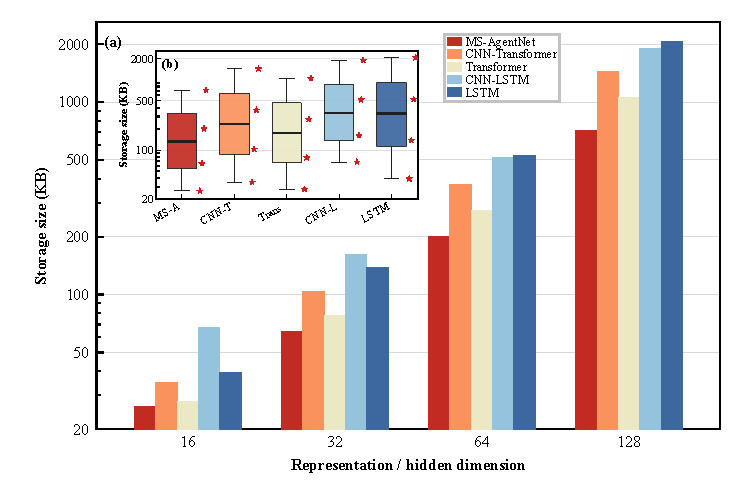
\includegraphics[width=0.78\linewidth]{figures/fig4_storage_scaling.pdf}
\caption{Storage sizes of different models.}
\label{fig:4-4}
\end{figure}


